%%
%% This is file `sample-sigconf.tex',
%% generated with the docstrip utility.
%%
%% The original source files were:
%%
%% samples.dtx  (with options: `all,proceedings,bibtex,sigconf')
%% 
%% IMPORTANT NOTICE:
%% 
%% For the copyright see the source file.
%% 
%% Any modified versions of this file must be renamed
%% with new filenames distinct from sample-sigconf.tex.
%% 
%% For distribution of the original source see the terms
%% for copying and modification in the file samples.dtx.
%% 
%% This generated file may be distributed as long as the
%% original source files, as listed above, are part of the
%% same distribution. (The sources need not necessarily be
%% in the same archive or directory.)
%%
%%
%% Commands for TeXCount
%TC:macro \cite [option:text,text]
%TC:macro \citep [option:text,text]
%TC:macro \citet [option:text,text]
%TC:envir table 0 1
%TC:envir table* 0 1
%TC:envir tabular [ignore] word
%TC:envir displaymath 0 word
%TC:envir math 0 word
%TC:envir comment 0 0
%%
%% The first command in your LaTeX source must be the \documentclass
%% command.
%%
%% For submission and review of your manuscript please change the
%% command to \documentclass[manuscript, screen, review]{acmart}.
%%
%% When submitting camera ready or to TAPS, please change the command
%% to \documentclass[sigconf]{acmart} or whichever template is required
%% for your publication.
%%
%%
\documentclass[nonacm,sigconf]{acmart}
%%
%% \BibTeX command to typeset BibTeX logo in the docs
\AtBeginDocument{%
  \providecommand\BibTeX{{%
    Bib\TeX}}}

%% Rights management information.  This information is sent to you
%% when you complete the rights form.  These commands have SAMPLE
%% values in them; it is your responsibility as an author to replace
%% the commands and values with those provided to you when you
%% complete the rights form.
% \setcopyright{acmlicensed}
\copyrightyear{2025}
\acmYear{2025}
% \acmDOI{XXXXXXX.XXXXXXX}
%% These commands are for a PROCEEDINGS abstract or paper.
\acmConference[Arxiv]{}{Nov}{2025}
%%
%%  Uncomment \acmBooktitle if the title of the proceedings is different
%%  from ``Proceedings of ...''!
%%
%%\acmBooktitle{Woodstock '18: ACM Symposium on Neural Gaze Detection,
%%  June 03--05, 2018, Woodstock, NY}
\acmISBN{}


%%
%% Submission ID.
%% Use this when submitting an article to a sponsored event. You'll
%% receive a unique submission ID from the organizers
%% of the event, and this ID should be used as the parameter to this command.
%%\acmSubmissionID{123-A56-BU3}

%%
%% For managing citations, it is recommended to use bibliography
%% files in BibTeX format.
%%
%% You can then either use BibTeX with the ACM-Reference-Format style,
%% or BibLaTeX with the acmnumeric or acmauthoryear sytles, that include
%% support for advanced citation of software artefact from the
%% biblatex-software package, also separately available on CTAN.

\usepackage{amsthm}
\newtheorem{definition}{Definition}

\usepackage{graphicx}  % for \resizebox
\usepackage{makecell}  % for line 
\usepackage{wrapfig}
\usepackage{subcaption}
\usepackage{siunitx} % For better number alignment, especially with ±
% 插入图片breaks inside table cells
% \usepackage{tikz}
 \usepackage{multirow}
\let\Bbbk\relax
\usepackage{amssymb} 
\usepackage{pifont}       % for \ding{55}
\usepackage{xcolor}       % for colored checkmark/xmark
\usepackage{rotating}   % 支持 sidewaysfigure
\usepackage{booktabs}   % 更美观的表格横线
\usepackage{adjustbox}  % 可选，缩放表格
\usepackage{algorithm}
\usepackage{algpseudocode}

% （可选）让输入/输出文字更漂亮
\renewcommand{\algorithmicrequire}{\textbf{Input:}}
\renewcommand{\algorithmicensure}{\textbf{Output:}}

%%
%% Look at the sample-*-biblatex.tex files for templates showcasing
%% the biblatex styles.
%%

%%
%% The majority of ACM publications use numbered citations and
%% references.  The command \citestyle{authoryear} switches to the
%% "author year" style.
%%
%% If you are preparing content for an event
%% sponsored by ACM SIGGRAPH, you must use the "author year" style of
%% citations and references.
%% Uncommenting
%% the next command will enable that style.
%%\citestyle{acmauthoryear}


%%
%% end of the preamble, start of the body of the document source.
\begin{document}

%%
%% The "title" command has an optional parameter,
%% allowing the author to define a "short title" to be used in page headers.
\title{Physically Interpretable World Models via \\ Weakly Supervised Representation Learning}

%%
%% The "author" command and its associated commands are used to define
%% the authors and their affiliations.
%% Of note is the shared affiliation of the first two authors, and the
%% "authornote" and "authornotemark" commands
%% used to denote shared contribution to the research.
% \author{Ben Trovato}
% \authornote{Both authors contributed equally to this research.}
% \email{trovato@corporation.com}
% \orcid{1234-5678-9012}
% \author{G.K.M. Tobin}
% \authornotemark[1]
% \email{webmaster@marysville-ohio.com}
% \affiliation{%
%   \institution{Institute for Clarity in Documentation}
%   \city{Dublin}
%   \state{Ohio}
%   \country{USA}
% }

% \author{Anonymous authors
% }
% \affiliation{%
%   \institution{Paper under double-blind review}
%   % \city{Hekla}
%   % \country{Iceland}
%   }
% \email{larst@affiliation.org}

\author{Zhenjiang Mao}
\affiliation{%
  \institution{University of Florida}
  \city{Gainesville}
  \country{USA}
}

\author{Mrinall Eashaan Umasudhan}
\affiliation{%
  \institution{University of Florida}
  \city{Gainesville}
  \country{USA}
}


\author{Ivan Ruchkin}
\affiliation{%
  \institution{University of Florida}
  \city{Gainesville}
  \country{USA}
}


% \author{Charles Palmer}
% \affiliation{%
%   \institution{Palmer Research Laboratories}
%   \city{San Antonio}
%   \state{Texas}
%   \country{USA}}
% \email{cpalmer@prl.com}

% \author{John Smith}
% \affiliation{%
%   \institution{The Th{\o}rv{\"a}ld Group}
%   \city{Hekla}
%   \country{Iceland}}
% \email{jsmith@affiliation.org}

% \author{Julius P. Kumquat}
% \affiliation{%
%   \institution{The Kumquat Consortium}
%   \city{New York}
%   \country{USA}}
% \email{jpkumquat@consortium.net}

%%
%% By default, the full list of authors will be used in the page
%% headers. Often, this list is too long, and will overlap
%% other information printed in the page headers. This command allows
%% the author to define a more concise list
%% of authors' names for this purpose.
\renewcommand{\shortauthors}{Mao et al.}

%%
%% The abstract is a short summary of the work to be presented in the
%% article.
\begin{abstract}
Learning predictive models from high-dimensional sensory observations is fundamental for cyber-physical systems, yet the latent representations learned by standard world models lack physical interpretability. This limits their reliability, generalizability, and applicability to safety-critical tasks. We introduce Physically Interpretable World Models (PIWM), a framework that aligns latent representations with real-world physical quantities and constrains their evolution through partially known physical dynamics. Physical interpretability in PIWM is defined by two complementary properties: (i) the learned latent state corresponds to meaningful physical variables, and (ii) its temporal evolution follows physically consistent dynamics. To achieve this without requiring ground-truth physical annotations, PIWM employs weak distribution-based supervision that captures state uncertainty naturally arising from real-world sensing pipelines. The architecture integrates a VQ-based visual encoder, a transformer-based physical encoder, and a learnable dynamics model grounded in known physical equations. Across three case studies (Cart Pole, Lunar Lander, and Donkey Car), PIWM achieves accurate long-horizon prediction, recovers true system parameters, and significantly improves physical grounding over purely data-driven models. These results demonstrate the feasibility and advantages of learning physically interpretable world models directly from images under weak supervision.
\end{abstract}

%%
%% The code below is generated by the tool at http://dl.acm.org/ccs.cfm.
%% Please copy and paste the code instead of the example below.
%%
\begin{CCSXML}
<ccs2012>
   <concept>
<concept_id>10010147.10010257.10010293.10010319</concept_id>
       <concept_desc>Computing methodologies~Learning latent representations</concept_desc>
       <concept_significance>500</concept_significance>
       </concept>
   <concept>
       <concept_id>10010520.10010553</concept_id>
       <concept_desc>Computer systems organization~Embedded and cyber-physical systems</concept_desc>
       <concept_significance>500</concept_significance>
       </concept>
 </ccs2012>
\end{CCSXML}

\ccsdesc[500]{Computing methodologies~Learning latent representations}
\ccsdesc[500]{Computer systems organization~Embedded and cyber-physical systems}

%%
%% Keywords. The author(s) should pick words that accurately describe
%% the work being presented. Separate the keywords with commas.
% \keywords{Do, Not, Use, This, Code, Put, the, Correct, Terms, for,
%   Your, Paper}

\keywords{Interpretable Representation Learning, Trajectory Prediction, World Models, Physics-Informed Machine Learning, Autonomous Systems}


%% A "teaser" image appears between the author and affiliation
%% information and the body of the document, and typically spans the
%% page.
% \begin{teaserfigure}
%   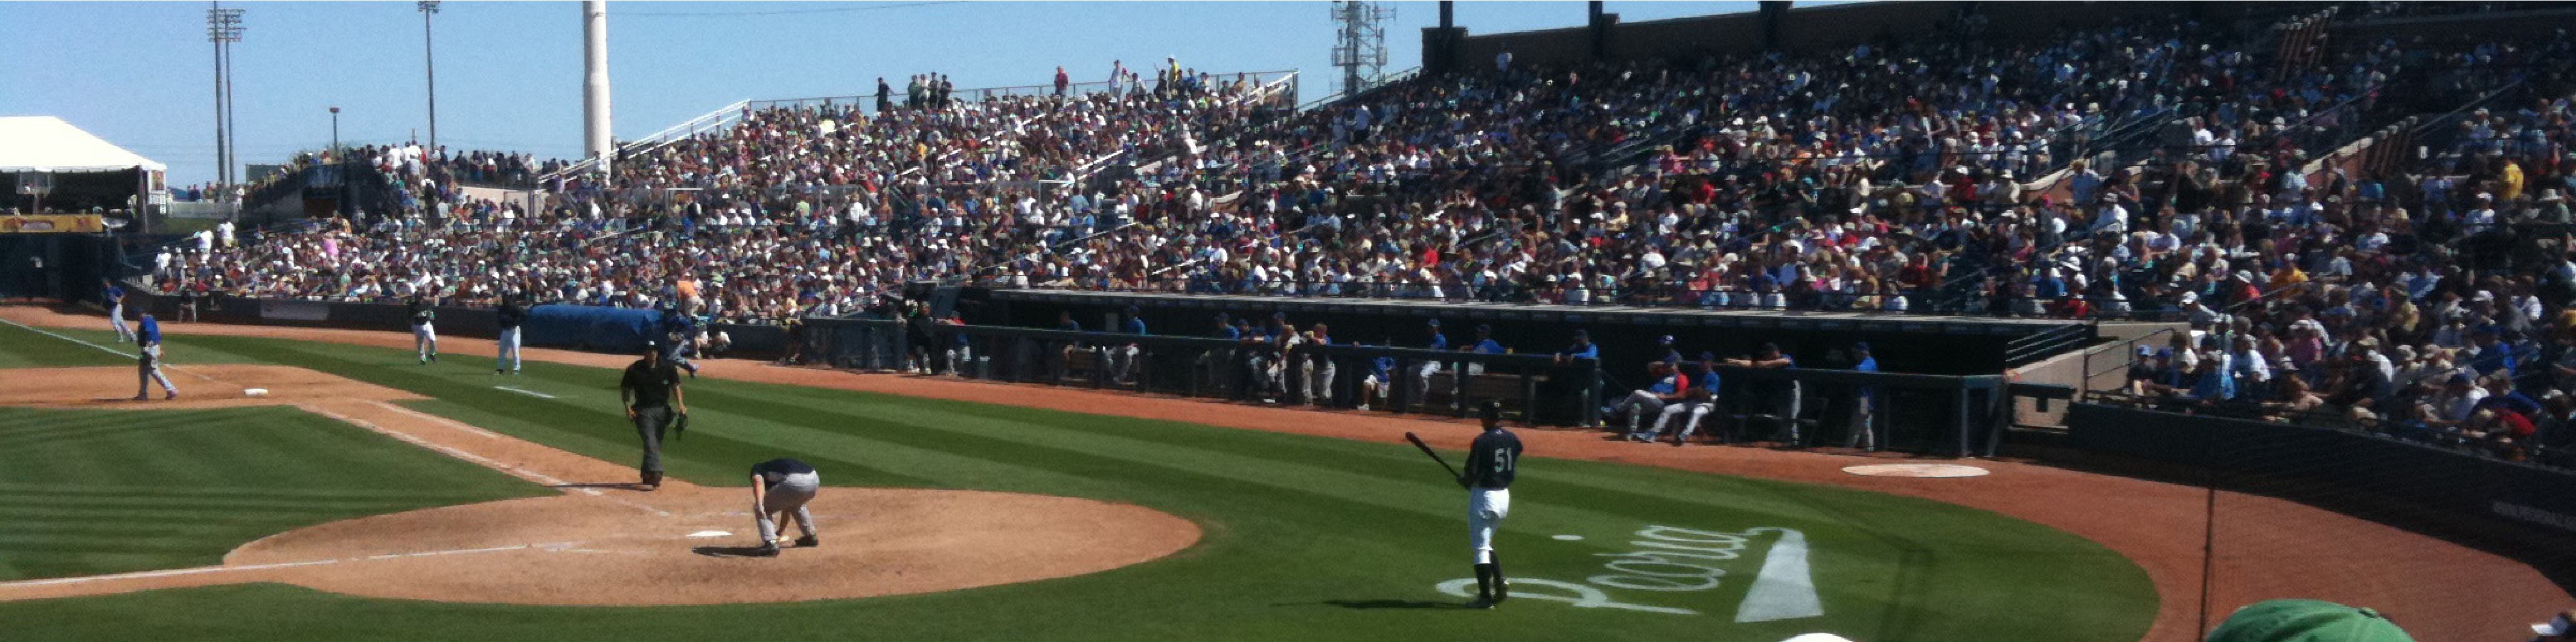
\includegraphics[width=\textwidth]{sampleteaser}
%   \caption{Seattle Mariners at Spring Training, 2010.}
%   \Description{Enjoying the baseball game from the third-base
%   seats. Ichiro Suzuki preparing to bat.}
%   \label{fig:teaser}
% \end{teaserfigure}

% \received{20 February 2025}
% \received[revised]{12 March 2009}
% \received[accepted]{5 June 2009}

%%
%% This command processes the author and affiliation and title
%% information and builds the first part of the formatted document.
\maketitle
\section{Introduction}

Accurate and robust trajectory prediction from high-dimensional sensor data, such as camera images, is a fundamental challenge for the safe operation of cyber-physical systems (CPS). A dominant paradigm for this task is to learn compact latent representations of the environment and evolve them over time. This idea underlies modern \textit{world models}~\cite{ha2018world}, which typically combine deep visual encoders with predictive temporal models such as RNNs or transformers~\cite{micheli2022transformers, hafner2023mastering, seo2023masked}. While these models achieve strong long-horizon prediction performance, their latent representations usually function as a ``black box,'' lacking a clear connection to the underlying physical state of the system.

Such a gap limits trustworthiness, controllability, and safety in CPS. In settings like autonomous driving or household robotics, physically meaningful latent states enable causal explanations (e.g., slowing down due to occlusions) and support high-assurance methodologies such as formal verification~\cite{hasan2015formal, katz2022verification} and run-time shielding~\cite{alshiekh2018safe, waga2022dynamic}. If predicted states can be mapped to interpretable quantities such as position or velocity, a safety monitor can detect unsafe future configurations (e.g., entering an occupied lane) and intervene accordingly. Furthermore, embedding physical structure into the latent space improves generalization by constraining predictions to physically plausible trajectories.

\looseness=-1
Existing attempts to learn physically interpretable latents from images generally fall into two paradigms, illustrated in Figure~\ref{fig:1}. \emph{Extrinsic} approaches first learn abstract visual latents and then map them to physical quantities via an additional model. \emph{Intrinsic} approaches instead attempt to encode physical structure directly within the image encoder, enforcing that the latent representation itself corresponds to meaningful physical variables. While effective in controlled settings~\cite{le2025pixie}, both paradigms typically \textit{require exact physical labels} during training or rely on object-centric decompositions~\cite{mosbach2025soldslotobjectcentriclatent}, which are difficult to reliably obtain from real-world CPS.


\looseness=-1
We aim to overcome this limitation by learning physical representations \emph{without exact physical supervision}. In many CPS, sensors such as GPS and radar naturally produce uncertain estimates in the form of distributions or confidence intervals rather than precise measurements. These distributional signals provide coarse yet informative constraints. For example, approximate position ranges or speed bounds that reflect the true physical state while tolerating noise and ambiguity. We leverage such distribution-based weak supervision to guide the encoding of high-dimensional images toward physically meaningful latent states. Combined with partially known system dynamics (which is also typical for CPS), this enables physically consistent multi-step prediction without requiring access to ground-truth states.


\begin{figure}[t] \centering 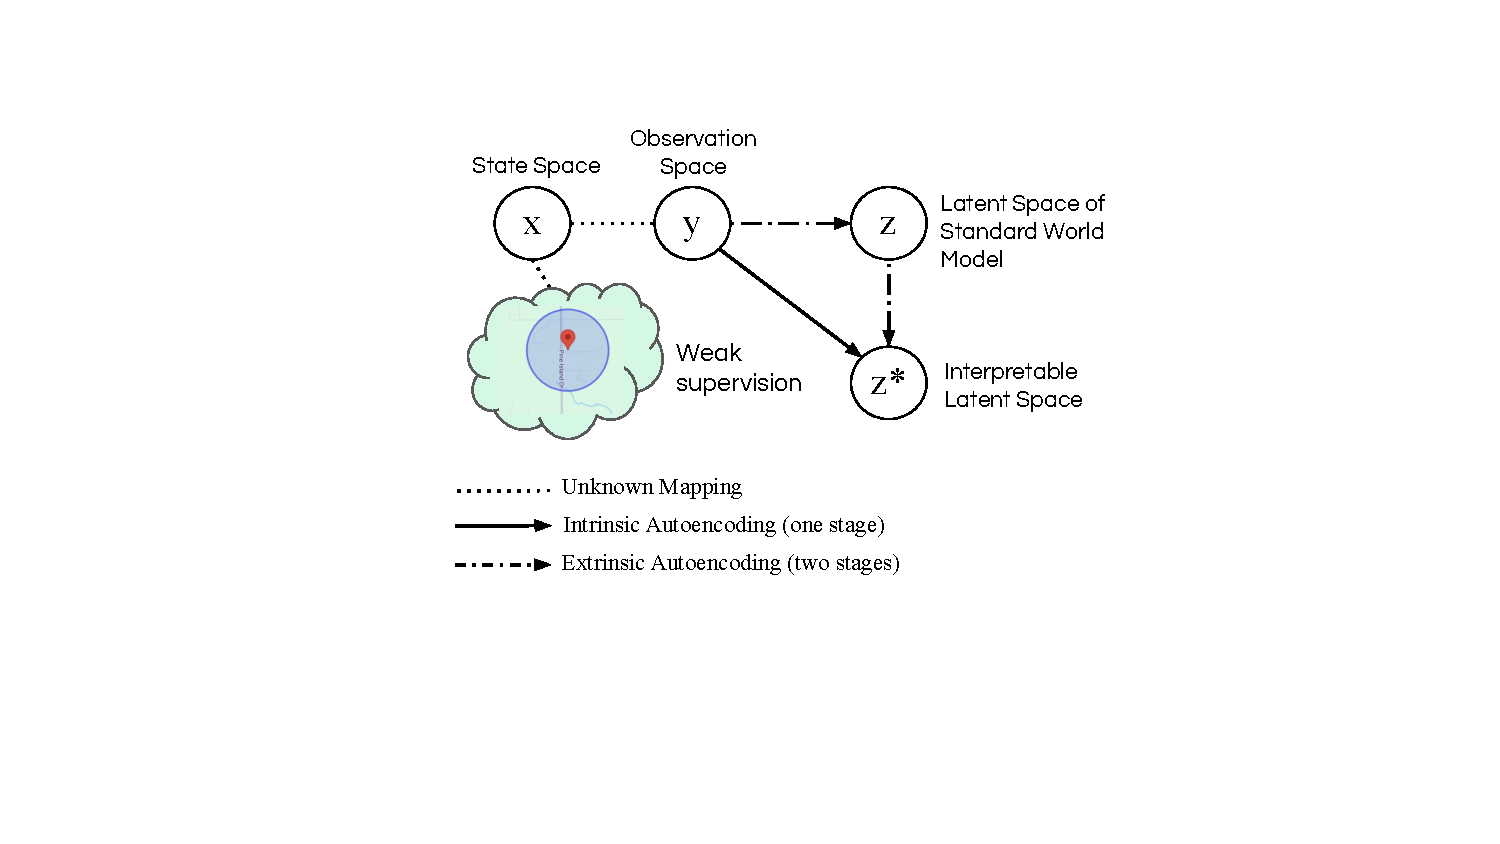
\includegraphics[width=0.9\columnwidth]{imgs/newoeverview.pdf} \caption{
Conceptual illustration of learning physically meaningful latent spaces from images.
High-dimensional observations $y$ may be encoded into a standard latent space $z$ or an interpretable latent space $z^*$.
Weak supervision vaguely relates observations to the underlying physical state $x$.
Existing approaches follow two paradigms: \emph{intrinsic} autoencoding (one-stage) and \emph{extrinsic} autoencoding (two-stage).
} \label{fig:1} \end{figure}

To this end, we propose the \textit{Physically Interpretable World Model (PIWM)}, a framework that learns latent states aligned with real physical quantities and constrains their temporal evolution using a structured, partially known dynamics model. In this work, \emph{physical interpretability} encompasses two complementary properties: (i) some latent dimensions correspond to meaningful physical variables, and (ii) latent evolution follows physically consistent dynamics. PIWM provides a general architectural template that combines image-based representation learning, physically interpretable latent spaces, and physics-informed dynamics.
Rather than prescribing a single architecture, PIWM defines a design space that can be instantiated with intrinsic or extrinsic encoders, and with continuous or discrete latent parameterizations.
Within this space, physical interpretability arises from aligning latent variables with weak supervision and constraining their temporal evolution through structured dynamics. Simultaneously, weak distributional supervision enforces alignment between latent states and physical quantities, eliminating reliance on the exact ground truth for training.

We conduct an extensive experimental study to answer a central question: \emph{How can weak supervision and latent quantization make world models physically interpretable?} We systematically examine continuous versus discrete latent spaces as well as intrinsic versus extrinsic designs. Across three case studies --- CartPole, Lunar Lander, and the DonkeyCar autonomous racing platform --- PIWM achieves superior physical grounding and long-horizon prediction accuracy compared to purely data-driven models and baselines. Notably, extrinsic architectures with quantized latent spaces consistently yield the most physically plausible and robust representations, highlighting the importance of decoupling visual encoding from physical interpretation.

Thus, this paper makes three contributions:
\begin{enumerate}
    \item \textbf{A unified definition of physical interpretability.}
    We formalize physical interpretability for generative world models as two complementary properties:
    (i) latent representations correspond to meaningful physical quantities, and
    (ii) their temporal evolution obeys physically valid dynamics.

    \item \textbf{A novel weakly supervised framework for learning physically grounded latents.}
    We introduce an architecture and training pipeline that aligns image-based latent states with physical variables using \emph{distribution-based weak supervision} instead of exact physical annotations. It also makes use of additional physical priors in the form of structural dynamics and latent quantization. % physical knowledge 

    % \item \textbf{A structured dynamics model that integrates partial physical knowledge.}
    % PIWM incorporates partially known second-order dynamics as architectural priors, learning only the unknown system parameters while ensuring physically plausible multi-step predictions.

    \item \textbf{A systematic empirical study of latent design choices.}
    Through extensive experiments on CartPole, Lunar Lander, and DonkeyCar, we analyze intrinsic vs.\ extrinsic architectures and continuous vs.\ discrete latents. The results reveal that \emph{extrinsic architectures with quantized latents} consistently achieve the most robust and interpretable representations, outperforming data-driven baselines in long-horizon prediction and physical parameter recovery.
\end{enumerate}

The remainder of this paper is organized as follows.
Section~\ref{sec:preliminaries} introduces the necessary background on autonomous systems, world models, and learned representations.
Section~\ref{sec:architecture} presents the proposed framework, including the representation learning module, the structured dynamics model, and the unified training procedure.
Section~\ref{sec:experiments} reports an extensive empirical study across three case studies, evaluating predictive performance, physical interpretability, and the effects of latent design choices. Section~\ref{sec:dis} discusses our findings, whereas Section~\ref{related} reviews the existing work.
Finally, Section~\ref{sec:conclusion} concludes the paper. 





\section{Preliminaries}\label{sec:preliminaries}

\subsection{Autonomous system and world models}
\begin{definition}[Autonomous CPS]
An \emph{autonomous CPS} $s = (X, I, Y, A, \phi_{\theta}, g, h)$ models the evolution of an perception-based control system, where the state set $X$ defines the finite-dimensional space of physical states, the initial set $I \subset X$ specifies possible starting states, observation set $Y$ contains all possible observations, and the action set $A$ contains available control actions. The system dynamics $\phi_{\theta}: X \times A \times \Theta \rightarrow X$ governs state transitions under physical parameters $\theta \in \Theta$, the observation function $g: X \rightarrow Y$ maps states to observations, and the fixed controller $h: Y \rightarrow A$ selects actions based on observations.
\end{definition}

We consider an autonomous system with observation-based control, the states of which evolve as $x_{t+1} = \phi(x_t, a_t, \theta^*),$ where $\theta^*$ are the true (unknown) physical parameters. The known controller $h$ relies on observations $y$ from sensors (e.g., cameras). Such controllers can be trained by imitation learning~\cite[]{hussein2017imitation} or reinforcement learning~\cite[]{kaelbling1996reinforcement,lillicrap2015continuous}, and we assume that it has been done for our purposes.
Given an initial state \( x_0 \in I \), a \textit{state trajectory} is defined by iteratively applying the dynamics function \( \phi \), yielding a sequence \( (x_0, x_1, \ldots, x_{i}) \), where each state is \( x_{t+1} = \phi(x_t, a_t, \theta^*) \) and the action is generated by the controller based on the observation:  \( a_{t}  = h(y_t) = h(g(x_t)) \). Correspondingly, an \textit{observation trajectory} \( (y_0, y_1, \ldots, y_{t}) \) is generated by applying the observation function \( g \) to each state: \( y_t = g(x_t) \). 


We consider the setting where the state is not directly observable, and to anticipate hazards and adapt, the system needs to forecast observations. This is done by combining a world model conditioned on past observations with an observation-based controller $h$, essentially forming an efficient online simulator of future observations. 

\begin{definition}[World Model]
A \emph{world model} $\mathcal{W} = (\mathcal{E}, f, \mathcal{D})$ predicts the future evolution of observations in an autonomous CPS $s$, where the encoder $\mathcal{E}: Y \rightarrow Z$ compresses high-dimensional observations into latent representations, the predictor $f: Z \times A \rightarrow Z$ forecasts future latents conditioned on actions, and the decoder $\mathcal{D}: Z \rightarrow Y$ reconstructs predicted observations. The actions $a_t$ are generated by a controller $h: Y \rightarrow A$ based on the current observation $y_t$, and together with the encoded latent $z_t = \mathcal{E}(y_t)$, are used to obtain the future latent $z_{t+1} = f(z_t, a_t)$. The predicted observation $\hat{y}_{t+1}$ is then obtained by decoding $z_{t+1}$ with $\mathcal{D}: \hat{y}_{t+1} = \mathcal{D}(z_{t+1}) $.
\end{definition}

While world models enable diverse tasks (e.g., controller training, monitoring, and planning), 
they are usually evaluated with \textit{predictive accuracy} --- how closely the predicted observations $\hat{y}_{t+1:t+n}$ match the true observations $y_{t+1:t+n}$. The typical metrics include mean squared error (MSE) and structural similarity index (SSIM). 
Unfortunately, these metrics are inherently limited: similar pixel-wise observations may correspond to very different underlying states. This means that the similarity (low MSE and high SSIM) between $\hat{y}_{t+1:t+n}$ and  $y_{t+1:t+n}$ does not guarantee similarity between the underlying physical states corresponding to the predicted observations and the true physical ones. Thus, the error in predicted observations is \textit{not physically interpretable}. This severely limits the predictions' utility for downstream CPS tasks like safety monitoring and planning. Instead, we turn our attention to the latent states. 

% \vspace{-2mm}
\subsection{Interpretable Latent Representations}

% \noindent
% \textbf{Variational Autoencoding.}

 \begin{figure*}[t]
	\centering     
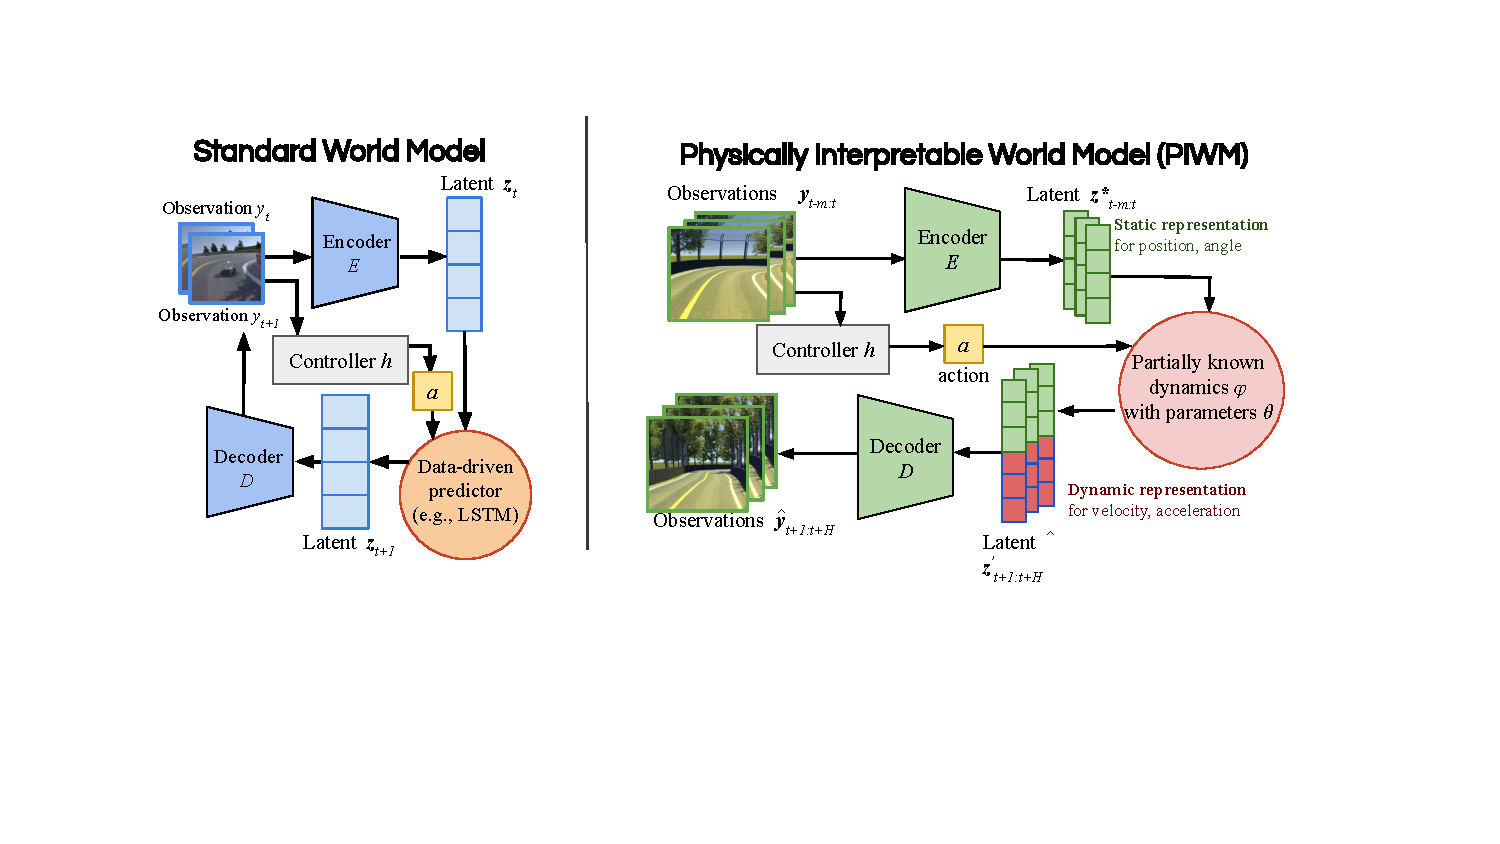
\includegraphics[width=1.7\columnwidth]{imgs/newcomp.pdf}
\caption{Overview of world model architectures. {(Left)}  Standard world model uses an encoder-decoder structure with a data-driven predictor (e.g., LSTM) to model latent dynamics, where the latent representations lack physical meaning. {(Right)} The PIWM architecture learns a structured latent representation $z^*$ from images, uses a learnable dynamics model $\phi$ with physical priors to predict future latent states, and decodes them into future images.}	\label{fig:15}
 \end{figure*}

 
The autoencoder components $\mathcal{E}$ and $\mathcal{D}$ in world models are primarily based on Variational Autoencoders (VAEs), Vector-Quantized Variational Autoencoder (VQ-VAEs), or their variants. VAEs~\cite[]{kingma2013auto} encode high-dimensional inputs \( y \) into continuous latent vectors \( z = \mathcal{E}(y) \), which are then decoded back into reconstructed inputs \( \hat{y} = \mathcal{D}(z) \). A standard VAE assumes a simple prior distribution over the latent space, typically an isotropic Gaussian, which facilitates tractable inference but imposes a strong inductive bias.  A VQ-VAE~\cite[]{van2017neural} discretizes the latent space by mapping a high-dimensional observation \( y_t \) to a continuous latent vector \( z_t = \mathcal{E}(y_t) \), then quantizing it via a \textit{codebook} \( \{\mathbf{e}_k\}_{k=1}^K \) to obtain a discrete latent \textit{index} \( z_t^* = \arg\min_k \|z_t - \mathbf{e}_k\|_2^2 \) closest to the continuous latent $z_t$. The decoder then reconstructs the observation via \( \hat{y}_t = \mathcal{D}(\mathbf{e}_{z_t^*}) \). While discretization introduces structure and regularization, the learned codebook vectors \( \mathbf{e}_k \) themselves are typically unstructured and lack interpretation.  Therefore, merely discretizing the space is insufficient: an explicit mechanism is needed to align these latent representations with physical semantics.



\looseness=-1
Our setting assumes that general knowledge about the dynamics function \( \phi \), namely the structure of its equations. However, the dynamics parameters \( \theta \), such as the mass or friction coefficient, are unknown, making the system $s$ only partially specified. In practice, it is often hard to find the true parameters $\theta^*$ because true physical states $x$ cannot be measured precisely. However, it is typical to compute a \textit{distribution} $p(x)$ from high-dimensional observations. For instance, the robot's pose may be estimated from images as a range/distribution --- and serve as a weak supervisory signal.

Thus, to train a world model, we are given a dataset \( \mathcal{S} \) of trajectories, consisting of \( N \) sequences of length \( M \), where each sequence contains tuples of images, actions, and state distribution labels:
\begin{equation}
 \mathcal{S} = \Big\{ \big(y_{1:M}, a_{1:M}, p_{1:M}(x) \big) \Big\}_{1:N}
\end{equation}

The weak supervision is provided by state distributions \( p_t(x) \), for which we assume no analytical form is known. Instead, we can only draw a finite set of samples from them. This represents a challenging yet practical scenario, as it is a weaker assumption than knowing the distribution's type (e.g., Gaussian), its parameters (e.g., mean and variance), or a definitive interval. 

\looseness=-1
Our ultimate task is to learn a representation \( z^* \) that accurately approximates the system’s true, unobserved physical state \( x \) for prediction. We formalize this as two distinct but related problems:

\begin{definition}[Interpretable Representation Learning Problem]
Given a dataset \( \mathcal{S} \) and a controller \( h \), the objective is to \emph{learn a state representation} \( z^* = \mathcal{E}(y) \) that minimizes the mean squared error to the true physical state \( x \):
\begin{equation}
\min_{\mathcal{E}} \ \mathbb{E} \big[ \| x - \mathcal{E}(y) \|_2^2 \big]
\end{equation}
\label{def:repprob}
\end{definition}

Next, the prediction problem is to forecast the evolution of these interpretable representations over time:

\begin{definition}[Prediction Problem for Interpretable Representations]
Given a dataset \( \mathcal{S} \), a dynamics function \( \phi \) with unknown parameters, and a controller \( h \), the objective is to \emph{train a predictor} that maps a history of representations to a future representation, \( \hat{z}^*_{t+H} = \mathcal{P}(z^*_{t-m:t}) \), by minimizing the future state prediction error:
\begin{equation}
\min_{\mathcal{P}} \ \mathbb{E} \big[ \| x_{t+H} - \hat{z}^*_{t+H} \|_2^2 \big].
\end{equation}
\label{def:predprob}
\end{definition}

The objectives in Definitions \ref{def:repprob} and \ref{def:predprob} are formulated with respect to the true physical state \( x \), which serves as the ultimate ground truth for evaluating physical interpretability. However, since \( x \) is not accessible during training, these objectives cannot be optimized directly. Our proposed method, detailed in Section~\ref{sec:architecture}, addresses this challenge by constructing a tractable surrogate objective that leverages the weak supervision by sampling state distributions \( p(x) \). Throughout this paper, we use calligraphic letters (e.g., $\mathcal{E}$, $\mathcal{D}$, $\mathcal{S}$) to denote functions and datasets for clarity. During training, we optimize model parameters $w$ using mini-batch gradient descent with batch size $B$, learning rate $\eta$, and train for $n_{\text{epochs}}$ epochs.


% \paragraph{Noise Model.}
% Let $\mathcal{S}_i = [x_i^{\min}, x_i^{\max}]$ denote the state space of the $i$-th physical dimension, and define its size as
% $\mathcal{X}_i = x_i^{\max} - x_i^{\min}$. 
% The weak supervision provides a nominal value $\mu_i$ for this dimension (e.g., the center of an interval estimate), but we assume that the true physical value $x_i$ is only known to lie in a neighborhood around $\mu_i$ whose width is proportional to the size of the state space:
% \[
%     x_i \in \big[\mu_i - \delta\, \mathcal{X}_i,\; \mu_i + \delta\, \mathcal{X}_i\big] \cap \mathcal{S}_i ,
% \]
% where $\delta \in (0,1)$ controls the uncertainty level of the weak supervision. 
% This interval-based noise model defines the feasible set $\Xi$ that is used in our weak supervision loss.


% The weak supervision in our formulation allows recovery of physical properties only through their influence on temporal evolution. 
% That is, a physical parameter is identifiable if and only if it induces observable differences in motion across a sequence of images. 
% Static appearance differences alone are insufficient: for instance, two objects with identical geometry but different mass or material remain distinguishable because they produce different trajectories under the same dynamics. 
% Thus, our method assumes that physical states are identifiable from motion, rather than from single-frame visual cues.


\paragraph{Noise Model.}
Since the true physical state $x$ is not directly observable, the weak
supervision available during training consists of samples drawn from an
unknown distribution $p(x)$ obtained from noisy sensor data.
We assume only that $p(x)$ provides a \emph{mean-proximal} estimate of each
state dimension. 
For the $i$-th state component, let $\mathcal{X}_i$ denote the valid 
range size of that dimension. Then the weak supervision is such that the true value $x_i$ lies within an 
interval of relative width~$\delta$ centered at the distributional mean:
\[
x_i \in 
\Big[
\mathbb{E}[p(x)] - \tfrac{1}{2}\delta\,|\mathcal{X}_i|,\;
\mathbb{E}[p(x)] + \tfrac{1}{2}\delta\,|\mathcal{X}_i|
\Big].
\]
Here, hyperparameter $\delta\in(0,1)$ quantifies the weakness of the supervision.  
This interval characterizes the feasible set from which supervision 
samples are drawn. In practice, we synthesize biased supervision noise to satisfy this assumption in Section~\ref{sec:setup}. It is important to distinguish our weak supervision from standard noisy-label supervised learning. First, PIWM never accesses the ground-truth state $x$ directly; it operates only on samples drawn from an unknown distribution $p(x)$. Second, no assumption is made about the analytical form or parameters of this distribution (e.g., we do not assume a Gaussian with known variance). Third, the interpretability objective aligns the latent state with the empirical mean of the sample set, not with a single corrupted regression target. This formulation reflects a more challenging and realistic scenario, as the model must infer the underlying state without any parametric description of the sensing noise.



\paragraph{Other assumptions.} 
Our method is designed under several standard and widely adopted assumptions for image-based CPS. First, we assume partial observability from images: the subset of physical variables we aim to recover is identifiable from a sequence of visual observations. Second, we adopt the Markovian system assumption, consistent with most world-model and control formulations: the next state depends only on the current state and action. Third, we assume that a partially known dynamics model provides a reasonable approximation of reality, but does not need to be exact.

% Observability from images, Markovian system, dynamics is a good approximation of reality (doesn't need to be true). Discuss future work in Sec DISCUSSION


\section{Architecture}\label{sec:architecture}

We introduce the \textit{Physically Interpretable World Model}, a flexible prediction architecture with physically-grounded representations of high-dimensional observations. It consists of two core components: (1) a {physically interpretable autoencoder} responsible for learning the state representation, and (2) a {learnable dynamics model} that predicts the evolution of this representation. A high-level overview of the proposed PIWM architecture is shown in Fig.~\ref{fig:15}, which contrasts it with a standard world model and highlights the structured, interpretable latent state. 

In our formulation, physical interpretability has two components. 
First, the learned physical latent variables $z^*$ correspond to meaningful physical quantities such as position, velocity, or other environment-specific state variables $x$. 
Second, the dynamics model $\phi$ learns to follow physically grounded evolution, ensuring that the temporal behavior of $z^*$ aligns with the underlying laws of motion. 
Our goal is to achieve both forms of interpretability directly from high-dimensional image observations under weak supervision. In our formulation, the physical state $x$ refers to a task-relevant, modeled subset of the full world state, namely the variables captured by the known dynamics equations $\phi$, such as position, velocity, and angle. Factors not captured by this subset (e.g., background motion, unmodeled friction) are not explicitly constrained by the symbolic dynamics and are instead implicitly absorbed into the visual components of the latent representation in both intrinsic and extrinsic variants.

\subsection{Learning Interpretable Representations}


The primary goal of the autoencoder is to map a high-dimensional observation \(y\) to a low-dimensional interpretable latent state \(z^*\). This representation must be explicitly aligned with the true physical state \(x\). Per Section~\ref{sec:preliminaries}, we cannot access \(x\) or the analytical form of its supervisory distribution \(p(x)\). Instead, we are given access to a set of \(L\) state proxy samples, \(\Xi = \{\xi^{(l)}\}_{l=1}^L\), drawn from \(p(x)\). To leverage these proxy samples \(\Xi\) for training, we formulate a general {interpretability loss}, \(\mathcal{L}_{\text{interp}}\), which measures the discrepancy between a predicted physically interpretable state \(z_p^*\) and the sample set \(\Xi\). In our experiments, we primarily use a Mean Squared Error (MSE) formulation that penalizes the distance to the empirical mean of the samples:
\begin{equation}
\mathcal{L}_{\text{interp}}(z_p^*, \Xi) = \| z_p^* - \hat{\mu}_{\xi} \|_2^2, \quad \text{where} \quad \hat{\mu}_{\xi} = \frac{1}{L}\sum_{l=1}^L \xi^{(l)}.
\label{eq:interp_loss}
\end{equation}
An alternative could be to use the Kullback-Leibler (KL) Divergence against a Gaussian fitted to the samples. This serves as the mechanism for enforcing physical grounding throughout our models.


\looseness=-1
A central design question in learning representation \(z^*\) is how to manage two competing objectives: reconstructing high-dimensional observations versus aligning the latent space with low-dimensional physical states. We consider two approaches, previously highlighted in Fig.~\ref{fig:1}. The \emph{Intrinsic} approach attempts to achieve both objectives simultaneously with a single, end-to-end encoder. While potentially more efficient, this forces one network to both capture fine-grained visual details (for reconstruction) and ignore those same details to extract the underlying physical state --- a difficult learning task. In contrast, the \emph{Extrinsic} approach follows a two-stage process: a vision autoencoder first learns an intermediate representation focused on reconstruction, and then a second, physical encoder extracts the interpretable state from it. This modularity may stabilize training but risks information loss in the intermediate step. Given the fundamental trade-offs, we will systematically investigate both approaches.

\looseness=-1
Orthogonal to this architectural choice, a second key design decision is the nature of the latent space \(Z^*\). \emph{Continuous spaces} can represent high-fidelity physical quantities but lack a built-in organizational prior, requiring explicit regularization for disentanglement. Conversely, \emph{discrete spaces} enforce regularity by design through their finite codebook but lose precision due to quantization error.
Below, we detail the combinations of intrinsic/extrinsic and continuous/discrete approaches. Note that the individual components, namely VAE/VQ-VAE encoders, $\beta$-VAE regularization, and second-order dynamics, are standard building blocks; the novelty of PIWM lies in their systematic integration with distribution-based weak supervision and the resulting design-space analysis.

\subsubsection{Intrinsic Autoencoding}

\looseness=-1
This approach employs a single, end-to-end encoder \(\mathcal{E}: Y \to Z^*\) that directly maps an observation \(y\) to the final interpretable latent state \(z^*\). This unified representation must disentangle visual features from physical semantics, a known challenge where information may leak between different physical attributes and hinder the desired learning \cite[]{peper2025four}.
For the case of \textit{continuous} latent space, the encoder outputs the parameters for a posterior distribution \(q(z^*\mid y)\) over the latent space \(Z^*\). Sampled from this distribution, a latent vector is then partitioned in a fixed manner:  \(z^* = [z_p^*, z_v^*]\), where \(z_p^*\) is the physically interpretable part and \(z_v^*\) captures the remaining visual information necessary for reconstruction. The full objective follows the \(\beta\)-VAE formulation, with the interpretability loss applied only to \(z_p^*\) and KL loss applied to $z_v^*$:
\begin{equation}
\begin{split}
    \mathcal{L}_{\text{intrinsic-cont}} = &\mathcal{L}_{\text{recon}}(y, \hat{y}) + \lambda_{\text{interp}}\mathcal{L}_{\text{interp}}(z_p^*, \Xi) \\
    &+ \beta D_{\text{KL}}\big(q(z_v^*|y) \,\|\, \mathcal{N}(0, I)\big)
\end{split}
\end{equation}


\looseness=-1
For the case of \textit{discrete} latent space, we structure the codebook to be interpretable. Each vector \(\mathbf{e}_k\) is partitioned as \(\mathbf{e}_k = [\mathbf{e}_k^p, \mathbf{e}_k^v]\).  Only the visual part \(\mathbf{e}_k^v\) is a typical learnable VQ-VAE codebook vector.  The physical part \(\mathbf{e}_k^p\) is a constant vector representing a specific point in a discretized grid of physical values (e.g., specific positions). Then, the interpretable state is computed as the average of the physical portions of the codebook vectors, \( z_p^* = \frac{1}{|I|} \sum_{i \in I} \mathbf{e}_i^p \). The full objective combines the standard VQ loss with our interpretability loss:
\begin{equation}
    \mathcal{L}_{\text{intrinsic-disc}} = \mathcal{L}_{\text{VQ}}(y, \hat{y}) + \lambda_{\text{interp}}\mathcal{L}_{\text{interp}}(z_p^*, \Xi),
\end{equation}
where \(\mathcal{L}_{\text{VQ}}\) includes reconstruction, codebook, and commitment losses:
\begin{equation}
    \mathcal{L}_{\text{VQ}} = \| y - \hat{y} \|_2^2 + \big\| \text{sg}[z_{\text{cont}}] - z_q \big\|_2^2 + \beta \big\| z_{\text{cont}} - \text{sg}[z_q] \big\|_2^2
\end{equation}


Here, \(z_{\text{cont}}\) is the continuous output of the encoder \(\mathcal{E}\), and \(z_q\) is its nearest vector from the codebook. The \(\text{sg}[\cdot]\) is the stop-gradient operator, which ensures that gradients are routed correctly for the codebook loss (updating \(z_q\)) and the commitment loss (updating \(z_{\text{cont}}\)). The hyperparameter \(\beta\) weights this commitment loss, controlling how strongly the encoder's output is encouraged to match the chosen codebook vector.


\subsubsection{Extrinsic Autoencoding}


This approach utilizes a two-stage training process to decouple perception from interpretation.
First, a general-purpose vision autoencoder (\(\mathcal{E}_v, \mathcal{D}_v\)) is trained to map an observation \(y\) to an intermediate latent vector \(z = \mathcal{E}_v(y)\). This stage is trained with a standard objective, independent of physical supervision.
For the \textit{continuous} case, this is a \(\beta\)-VAE trained to minimize:
\begin{equation}
    \mathcal{L}_{\text{vision-cont}} = \mathcal{L}_{\text{recon}}(y, \hat{y}) + \beta D_{\text{KL}}\big(q(z \mid y) \,\|\, \mathcal{N}(0, I)\big)
\end{equation}
For the \textit{discrete} case, a VQ-VAE is trained to minimize the standard VQ loss \(\mathcal{L}_{\text{vision-disc}} = \mathcal{L}_{\text{VQ}}(y, \hat{y})\).


After the first stage, the vision encoder \(\mathcal{E}_v\) is frozen. The second stage trains a separate, auxiliary {physical autoencoder} (\(\mathcal{E}_p, \mathcal{D}_p\)) to map the intermediate representation \(z = \mathcal{E}_v(y)\) to a final, purely physical representation \(z^* = \mathcal{E}_p(z)\). The training objective for this stage is:
\begin{equation}
    \mathcal{L}_{\text{physical}} = \lambda_{\text{interp}}\mathcal{L}_{\text{interp}}(z^*, \Xi) + \lambda_{\text{latent}}\mathcal{L}_{\text{recon}}\big(z,  \mathcal{D}_p(z^*))
\end{equation}

This same loss \(\mathcal{L}_{\text{physical}}\) is used for both continuous and discrete intermediate representation \(z\). Additional architectural diagrams of the 
extrinsic--discrete pipeline are provided in the extended version~\cite{extended} for clarity.


\begin{algorithm}[t]
\caption{
Training pipeline for PIWM. Models are trained in separate stages, freezing the
parameters of earlier stages before optimizing the next one.
}
\label{alg:piwm}
\begin{algorithmic}[1]

\Require Training set $\mathcal{S}$, batch size $B$, weights $\{\lambda_i\}$

% ---------------------- Stage 1 ------------------------
\State \textbf{// Stage 1: Train the vision autoencoder (extrinsic only)}
\If{architecture = extrinsic}
    \For{epoch $= 1$ to $n_{\text{vision}}$}
      \For{each batch of $(y_t)$}
        \State $z_t \gets \mathcal{E}_v(y_t)$
        \If{latent = discrete}
            \State $z_t \gets \text{Quantize}(z_t)$
        \EndIf
        \State $\hat{y}_t \gets \mathcal{D}_v(z_t)$
        \State $\mathcal{L}_{\text{vision}} \gets 
               \mathcal{L}_{\text{rec}}(y_t, \hat{y}_t) 
               + \lambda_3 \mathcal{L}_{\text{reg}}$
        \State Update $(\mathcal{E}_v, \mathcal{D}_v)$ using 
               $\nabla \mathcal{L}_{\text{vision}}$
      \EndFor
    \EndFor
    \State Freeze parameters of $\mathcal{E}_v$
\EndIf

% ---------------------- Stage 2 ------------------------
\State \textbf{// Stage 2: Train the physical encoder–decoder}
\For{epoch $= 1$ to $n_{\text{physical}}$}
  \For{each batch of $(y_t, \Xi_t)$}
    \If{architecture = intrinsic}
        \State $z^*_t \gets \mathcal{E}(y_t)$
    \Else
        \State $z_t \gets \mathcal{E}_v(y_t)$
        \If{latent = discrete}
            \State $z_t \gets \text{Quantize}(z_t)$
        \EndIf
        \State $z^*_t \gets \mathcal{E}_p(z_t)$
    \EndIf
    \State Compute interpretability loss 
           $\mathcal{L}_{\text{interp}}(z^*_t, \Xi_t)$
    \If{architecture = extrinsic}
        \State $\hat{z}_t \gets \mathcal{D}_p(z^*_t)$
        \State $\mathcal{L}_{\text{latent-rec}} \gets 
               \|z_t - \hat{z}_t\|^2$
    \Else
        \State $\mathcal{L}_{\text{latent-rec}} \gets 0$
    \EndIf
    \State $\mathcal{L}_{\text{phys}} \gets 
           \lambda_1 \mathcal{L}_{\text{interp}}
           + \lambda_2 \mathcal{L}_{\text{latent-rec}}$
    \State Update physical encoder–decoder using $\nabla \mathcal{L}_{\text{phys}}$
  \EndFor
\EndFor
\State Freeze $\mathcal{E}$ (intrinsic) or $(\mathcal{E}_p, \mathcal{D}_p)$ (extrinsic)

% ---------------------- Stage 3 ------------------------
\State \textbf{// Stage 3: Train the dynamics model}
\For{epoch $= 1$ to $n_{\text{dyn}}$}
  \For{each batch of $(y_{t:t+2}, a_t, \Xi_{t:t+2})$}
    \State Encode states to obtain $z^*_t$, $z^*_{t+1}$
    \State Predict next physical state 
           $\hat{z}^*_{t+2} \gets \phi_\theta(z^*_t, z^*_{t+1}, a_t)$
    \State Compute dynamics loss 
           $\mathcal{L}_{\text{dyn}}(\hat{z}^*_{t+2}, \Xi_{t+2})$
    \State Update $\theta$ using $\nabla \mathcal{L}_{\text{dyn}}$
  \EndFor
\EndFor

\State \Return trained model parameters
\end{algorithmic}
\end{algorithm}



% \begin{algorithm}[t]
% \caption{
% Training pipeline for PIWM. Models are 
% trained in separate stages, freezing the parameters of the previous stage 
% before beginning the next one.
% }
% \label{alg:piwm}
% \begin{algorithmic}[1]
% \Require Training set $\mathcal{S} = \{(y_{1:M}, a_{1:M}, \Xi_{1:M})\}_{i=1}^N$, architecture type, latent type, batch size $B$, weights $\{\lambda_i\}$
% \Ensure Trained model parameters $w$
% \State Initialize model parameters $w$ randomly
% \For{epoch $= 1$ to $n_{\text{epochs}}$}
%   \For{each batch of $B$ sequences from $\mathcal{S}$}
%     \For{$t = 1$ to $M - 2$}
%       \State \textbf{Stage 1: Encode observations to latent space}
%       \If{architecture = intrinsic}
%         \State $z^*_t \gets \mathcal{E}(y_t)$; \quad $z^*_{t+1} \gets \mathcal{E}(y_{t+1})$
%         \If{latent = discrete}
%           \State $z^*_t \gets \text{Quantize}(z^*_t)$
%         \EndIf
%         \State $z^*_p[t] \gets \text{ExtractPhysical}(z^*_t)$
%       \Else
%         \State $z_t \gets \mathcal{E}_v(y_t)$; \quad $z_{t+1} \gets \mathcal{E}_v(y_{t+1})$
%         \If{latent = discrete}
%           \State $z_t \gets \text{Quantize}(z_t)$
%         \EndIf
%         \State $z^*_p[t] \gets \mathcal{E}_p(z_t)$
%       \EndIf
      
%       \State \textbf{Stage 2: Predict dynamics}
%       \State $a_t \gets h(y_t)$
%       \State $\hat{z}^*_p[t+2] \gets \phi_\theta(z^*_p[t], z^*_p[t+1], a_t)$
      
%       \State \textbf{Stage 3: Decode for reconstruction}
%       \If{architecture = intrinsic}
%         \State $\hat{y}_{t+2} \gets \mathcal{D}(\text{Combine}(\hat{z}^*_p[t+2], z^*_v[t+2]))$
%       \Else
%         \State $\hat{z}_{t+2} \gets \mathcal{D}_p(\hat{z}^*_p[t+2])$
%         \State $\hat{y}_{t+2} \gets \mathcal{D}_v(\hat{z}_{t+2})$
%       \EndIf
      
%       \State \textbf{Stage 4: Compute losses}
%       \State $\mathcal{L}_{\text{rec}} \gets \|y_{t+2} - \hat{y}_{t+2}\|^2_2$
%       \State $\mathcal{L}_{\text{interp}} \gets \text{InterpLoss}(z^*_p[t], \Xi_t)$
%       \State $\mathcal{L}_{\text{dyn}} \gets \text{InterpLoss}(\hat{z}^*_p[t+2], \Xi_{t+2})$
      
%       \If{latent = continuous}
%         \State $\mathcal{L}_{\text{reg}} \gets \beta \cdot D_{KL}(q(z|y) \| p(z))$
%       \Else
%         \State $\mathcal{L}_{\text{reg}} \gets \mathcal{L}_{\text{VQ}} + \mathcal{L}_{\text{commit}}$
%       \EndIf
      
%       \State $\mathcal{L} \gets \mathcal{L}_{\text{rec}} + \lambda_1 \mathcal{L}_{\text{interp}} + \lambda_2 \mathcal{L}_{\text{dyn}} + \lambda_3 \mathcal{L}_{\text{reg}}$
%     \EndFor
%     \State Update parameters: $w \gets w - \eta \nabla_w \mathcal{L}$
%   \EndFor
% \EndFor
% \State \Return $w$
% \end{algorithmic}
% \end{algorithm}


 
\subsection{Learnable Dynamics Model}

% \textbf{Learnable Dynamics Model.}

The second core component of our PIWM is a latent dynamics model \(\phi\) that predicts the temporal evolution of the physically interpretable state \(z^*\). Rather than using black-box sequence models, our prediction is based on known dynamics equations, \(\phi(z^*_t, a_t, \theta)\), where the form of \(\phi\) (e.g., kinematics) is fixed and only its parameters \(\theta\) are learnable. This allows our model to reflect the underlying physical laws while adapting to unknown system parameters $\theta$ such as friction and mass.

The dynamics model is responsible for estimating physical quantities that depend on a history of states, such as velocity, in order to predict the system's evolution. 
To do this, the model is initialized with a short window of consecutive representations, \( (z^*_t, z^*_{t+1}) \), produced by the encoder from observations. 
These two states, along with the control action \(a_{t+1}\) that causes the transition from state \(t+1\) to \(t+2\), are used by the learnable dynamics model \(\phi\) to predict the next state: \( \hat{z}^*_{t+2} = \phi(z^*_t, z^*_{t+1}, a_{t+1}, \theta) \). 
By taking two consecutive states as input, the model can internally compute velocity and other time-derivative quantities necessary for an accurate physical prediction. This method can be extended to higher-order derivatives with more consecutive inputs.
After this initialization phase, the model can operate recursively for multi-step rollouts, taking its own prediction from the previous step as input to generate a future trajectory. 
This enables efficient, long-horizon forecasting without needing a sequence of observations at every step.

\looseness=-1
The parameters \(\theta\) of the dynamics model \(\phi\) are learned by minimizing a dynamics loss, \(\mathcal{L}_{\text{dyn}}\). This objective ensures that the predicted state \(\hat{z}^*_{t+H}\), generated by recursively applying the dynamics model \(\phi(\cdot, \cdot, \theta)\), aligns with the weak supervision available for that future time step. We use a Mean Squared Error (MSE) loss, which compares the prediction against the empirical mean of the proxy labels \(\Xi_{t+H}\). The loss is defined as a function of the parameters \(\theta\):
\begin{equation}
    \mathcal{L}_{\text{dyn}}(\theta) = \| \hat{z}^*_{t+H} -  \hat{\mu}_{\xi_{t+H}} \|_2^2,
\end{equation}
where $\hat{z}^*_{t+H}$ is the state predicted by the dynamics model parameterized by $\theta$, and $\hat{\mu}_{\xi_{t+H}} = \frac{1}{L}\sum_{l=1}^L \xi^{(l)}_{t+H}$ is the empirical mean of the $L$ proxy samples for the future state. 


To optimize the learnable parameters $\theta$, we backpropagate 
through the structured \emph{second-order} dynamics model used in Algorithm~\ref{alg:piwm}.
Since each predicted state $\hat{z}^{*}_{t+H}$ is obtained by recursively applying
\begin{equation}
\hat{z}^{*}_{t+2} = \phi(z^{*}_{t},\, z^{*}_{t+1},\, a_{t+1};\, \theta),
\end{equation}
it depends on \emph{two} previous latent states, consistent with the model definition.
The gradient of the multi-step dynamics loss is:
\begin{equation}
\frac{\partial \mathcal{L}_{\mathrm{dyn}}}{\partial \theta}
=
\frac{\partial \mathcal{L}_{\mathrm{dyn}}}{\partial \hat{z}^{*}_{t+H}}
\cdot
\frac{\partial \hat{z}^{*}_{t+H}}{\partial \theta}.
\end{equation}

The recursive derivative for $\hat{z}^{*}_{t+H}$ expands as:
\begin{equation}
\frac{\partial \hat{z}^{*}_{t+H}}{\partial \theta}
=
\frac{\partial \phi}{\partial \theta}
+
\frac{\partial \phi}{\partial z^{*}_{t+H-1}}
\cdot
\frac{\partial z^{*}_{t+H-1}}{\partial \theta}
+
\frac{\partial \phi}{\partial z^{*}_{t+H-2}}
\cdot
\frac{\partial z^{*}_{t+H-2}}{\partial \theta},
\end{equation}
reflecting the fact that the dynamics model $\phi$ takes 
$$(z^{*}_{t+H-2}, z^{*}_{t+H-1}, a_{t+H-1})$$ as inputs.
This recursive computation enables end-to-end learning of both the interpretable 
latent states and the dynamics parameters, ensuring that the learned physical 
parameters remain consistent with observed trajectories. During training, the dynamics model is optimized after the representation
modules have been trained and frozen.








\begin{figure*}[t]
	\centering         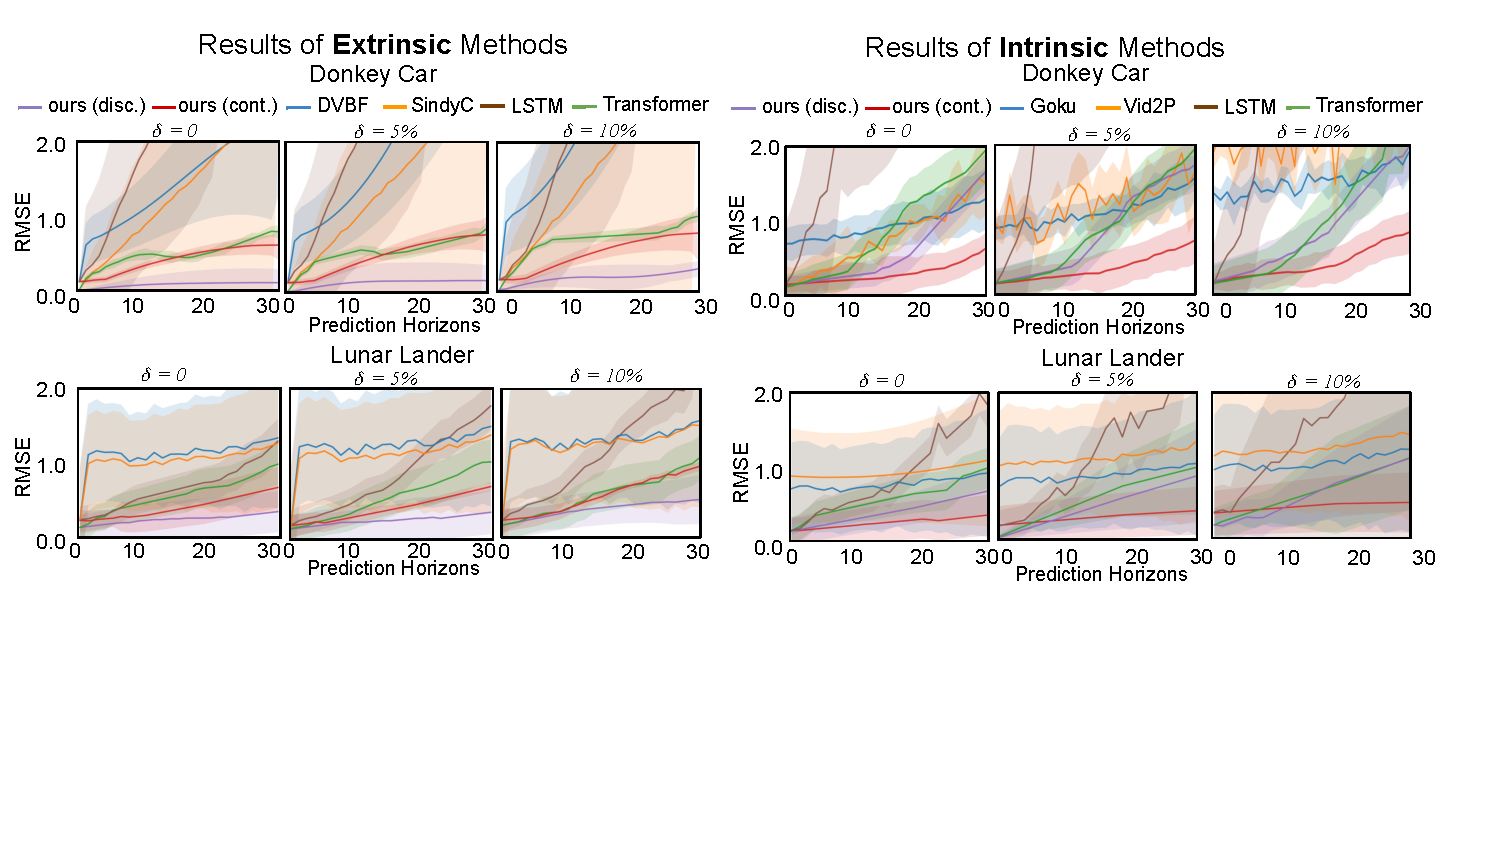
\includegraphics[width=1.8\columnwidth]{imgs/resultsx2.pdf}
\caption{Prediction performance. The Root Mean Square Error (RMSE) of our PIWM variants (extrinsic methods, left; intrinsic methods, right) is compared against baselines over a 30-step prediction horizon in the Donkey Car and Lunar Lander across varying levels of weak supervision ($\delta$).}	\label{fig:2}

 \end{figure*}

 
\subsection{Training Procedure}

PIWM is not trained end-to-end for all variants. 
Intrinsic and models are trained 
in two and three stages: the vision autoencoder is trained first and then frozen; 
the physical encoder–decoder is trained next and then frozen (only for extrinsic one); 
finally, the dynamics model is trained with both encoders fixed. 
Algorithm~\ref{alg:piwm} summarizes the staged training procedure. The total loss combines $\mathcal{L}_{\text{rec}}$, $\mathcal{L}_{\text{interp}}$, $\mathcal{L}_{\text{dyn}}$, and $\mathcal{L}_{\text{reg}}$; only the relevant components are active in each stage.

% Algorithm~\ref{alg:piwm} illustrates the unified forward pass, while the actual 
% optimization for extrinsic models follows this staged schedule.
% Algorithm~\ref{alg:piwm} therefore describes a conceptual per-timestep update,
% while the actual optimization is performed using this staged schedule.
% Algorithm~\ref{alg:piwm} summarizes our unified training framework for PIWM, which integrates the learning of interpretable representations with dynamics modeling. The training operates on a dataset $$\mathcal{S} = \{(y_{1:M}, a_{1:M}, \Xi_{1:M})\}_{i=1}^N,$$ consisting of $N$ trajectories, where each trajectory contains $M$ time steps of observations $y$, actions $a$, and weak supervision samples $\Xi$. The model parameters $w$ are optimized using mini-batch gradient descent with batch size $B$ and learning rate $\eta$ over $n_{\text{epochs}}$ epochs.

% The training follows a four-stage process within each time step:

% \noindent
% \textbf{Stage 1: Encoding.} For intrinsic architectures, observations are directly encoded to interpretable states $z^*$ via encoder $\mathcal{E}$. For extrinsic architectures, a two-stage process first encodes observations to intermediate representations $z$ using vision encoder $\mathcal{E}_v$, then maps them to physical states $z^*_p$ via physical encoder $\mathcal{E}_p$. Discrete variants apply quantization after encoding.

% \noindent
% \textbf{Stage 2: Dynamics Prediction.} The learnable dynamics model $\phi_\theta$ takes two consecutive physical states $z^*_p[t], z^*_p[t+1]$ and action $a_t = h(y_t)$ from controller $h$ to predict the next state $\hat{z}^*_p[t+2]$. This enables the model to internally compute velocities and other derivatives necessary for physical prediction.

% \noindent
% \textbf{Stage 3: Decoding.} Intrinsic models decode by combining predicted physical states with visual features. Extrinsic models first decode to intermediate representations via $\mathcal{D}_p$, then to observations via $\mathcal{D}_v$.


% The total loss combines reconstruction error $\mathcal{L}_{\text{rec}}$, interpretability alignment $\mathcal{L}_{\text{interp}}$ with weak supervision $\Xi$, dynamics prediction accuracy $\mathcal{L}_{\text{dyn}}$, and regularization $\mathcal{L}_{\text{reg}}$ (KL divergence for continuous, VQ losses for discrete). Only the relevant components of the loss are active in each training stage.

% The key distinction from standard world models lies in the explicit alignment of latent representations with physical quantities through weak supervision and physical priors, to support both accurate prediction and physical interpretability.

\section{Experimental Evaluation}\label{sec:experiments}
To validate our PIWM approach, we experiment on three environments: CartPole, Lunar Lander, and the DonkeyCar autonomous racing platform~\cite[]{brockman2016openai,viitala2021learning}. These environments differ in the observation dimensionality, action space, and underlying dynamics.

% \noindent
% \textbf{Experimental Setup.}

\subsection{Experimental Setup}\label{sec:setup}

For each environment, we collect a dataset of 60,000 trajectories, each with at least 50 time steps. To ensure diverse state space coverage, trajectories are generated by executing both random actions and those generated by well-trained neural controllers. 

The weak supervision labels used in all experiments instantiate the 
uniform-distribution noise model described in Sec.~\ref{sec:preliminaries}.  
In practice, this means that the supervisory distribution $p(x)$ for
each state dimension is implemented as a biased uniform distribution over a 
bounded interval of relative width~$\delta$.  For each ground-truth 
state component $x_i$, let $\mathcal{X}_i$ denote the valid 
range size of that dimension.  We first generate a randomly shifted 
center:
\[
\tilde{\mu}_i 
= x_i + \Delta_i,
\qquad 
\Delta_i \sim \mathrm{Unif}\!\left[
    -\tfrac{1}{2}\delta \,|\mathcal{X}_i|,\;
    \tfrac{1}{2}\delta \,|\mathcal{X}_i|
\right].
\]
We then define the supervisory distribution itself as a uniform
distribution supported on an interval of the same width:
\[
p_i(x) = \mathrm{Unif}\!\left[
\tilde{\mu}_i - \tfrac{1}{2}\delta\,|\mathcal{X}_i|,\;
\tilde{\mu}_i + \tfrac{1}{2}\delta\,|\mathcal{X}_i|
\right].
\]
At each time step, we draw $50$ samples from this distribution to form 
the proxy supervision set $\Xi$ used in training.





% The weak supervision signals are generated by perturbing the ground-truth physical states for different noise levels $\delta \in \{0, 5\%, 10\%\}$. For each, the weak supervision given by a uniform distribution over an interval constructed as follows. Its width is equal to the \(\delta\) fraction of the full range of the respective state dimension. The interval's center is randomly shifted from the ground truth by an amount drawn from a uniform distribution over \([-\delta/2 \mathcal{X}, \delta/2 \mathcal{X}]\) of the full state range.

For the experiments, our vision encoder $\mathcal{E}_v$ uses two convolutional layers with channel projection to a 64-dimensional latent space. Discrete variants employ a 512-entry codebook with commitment loss weight $\beta = 0.25$. The physical encoder $\mathcal{E}_p$ is a 2-layer Transformer (4 heads, 512 feedforward dimension) with mean pooling and linear projection to physical states. The decoder $\mathcal{D}_p$ mirrors this architecture. 
We apply early stopping based on validation loss to prevent overfitting and to ensure stable convergence across environments. 
In addition, we use a cosine learning-rate decay schedule, which improves long-horizon rollout stability for the second-order latent dynamics model. 
These training settings follow standard practices in world-model and VQ-VAE training. 
We performed a small-scale sweep over candidate learning rates and regularization magnitudes and selected the configuration that yielded stable reconstruction loss, non-diverging rollouts, and consistent convergence across datasets. More details can be found in the extended version~\cite{extended}. To ensure a fair comparison, all baselines are implemented following their original publications or official codebases and trained under identical settings: the same dataset, rollout horizon, optimizer (Adam), learning rate schedule, and early stopping criterion based on validation loss. No additional hyperparameter tuning was performed exclusively for PIWM; all configuration choices were made on a held-out validation split shared across all models.



\begin{figure}[t]
	\centering         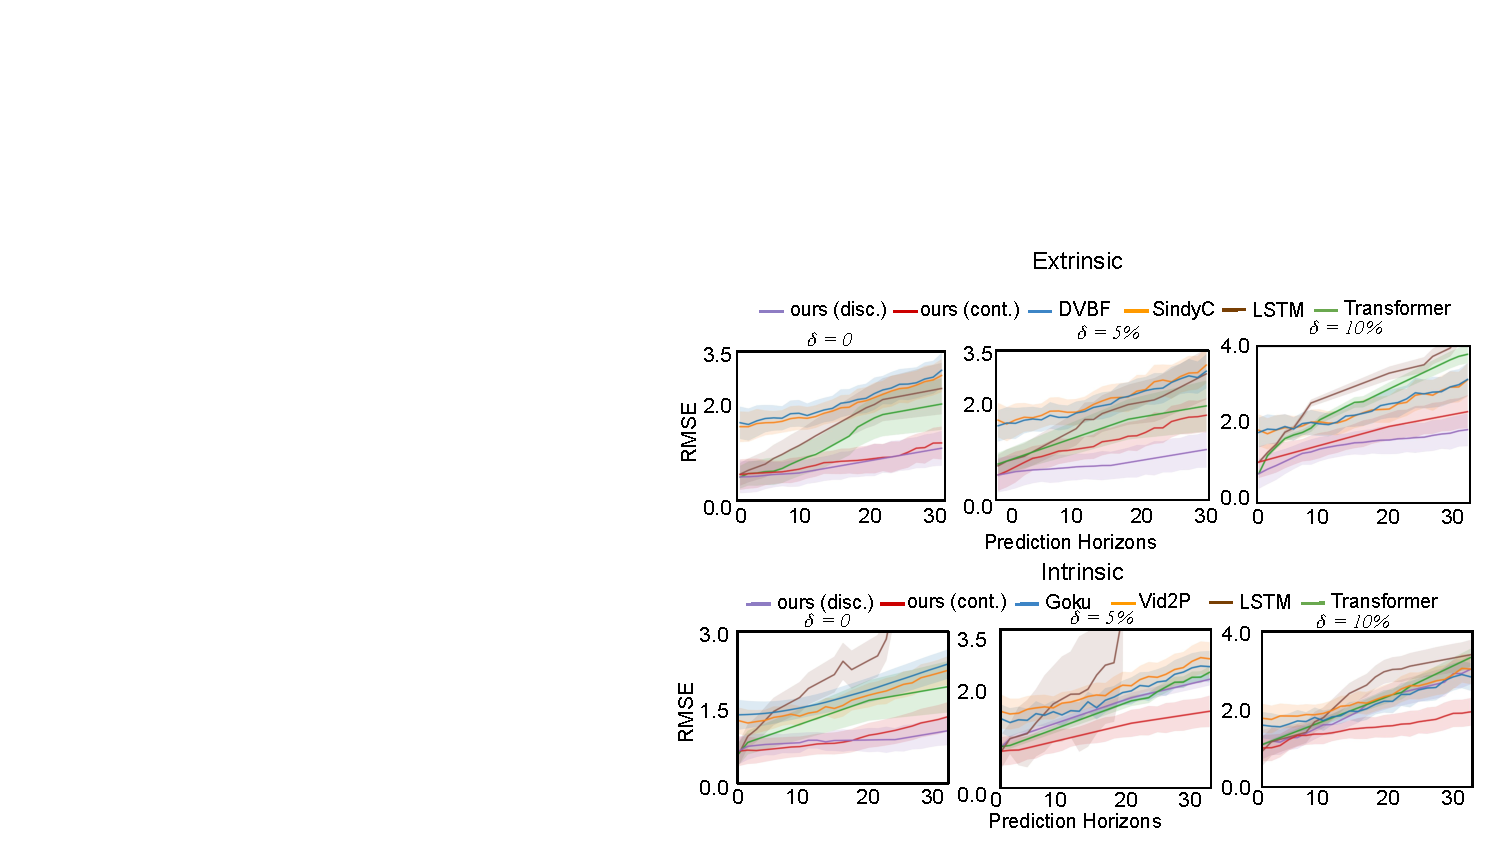
\includegraphics[width=\columnwidth]{imgs/cartresults.pdf}
\caption{Prediction performance of CartPole. The Root Mean Square Error (RMSE) of our PIWM variants (extrinsic methods, upper; intrinsic methods, lower) is compared against baselines over a 30-step prediction horizon in the CartPole across varying levels of weak supervision ($\delta$).}	\label{fig:para}
 \end{figure}


 \begin{figure*}[t]
  \centering
  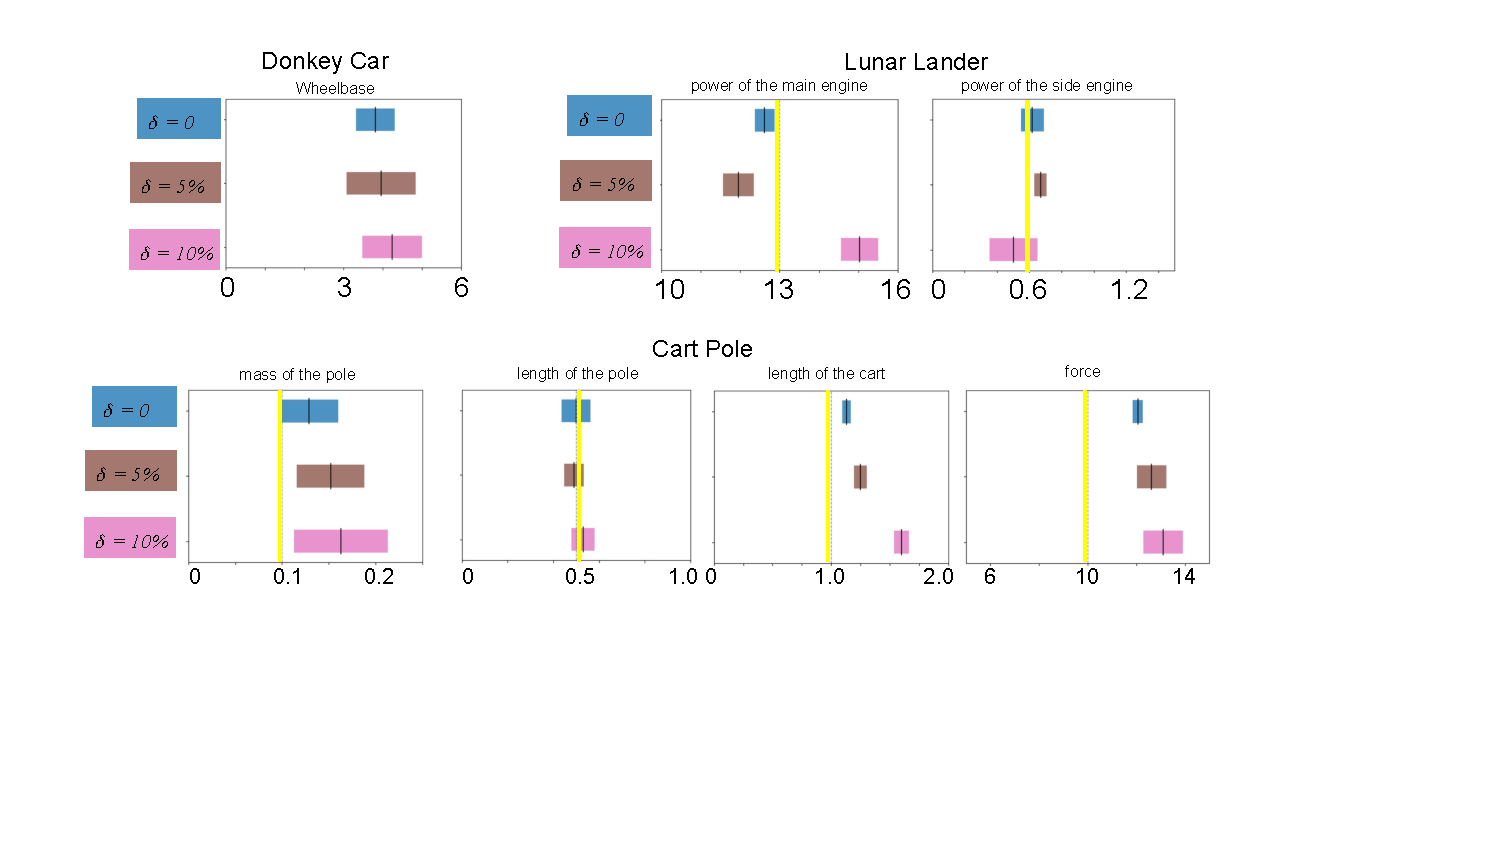
\includegraphics[width=0.83\textwidth]{imgs/allpara.pdf} 
\caption{
Learned physical parameters vs.\ ground truth. 
For Cart Pole and Lunar Lander, the parameters learned by our model 
(colored bars) are compared against the known ground-truth values 
(yellow lines) under varying noise levels ($\delta$). 
For the Donkey~Car, we use only an approximate bicycle model 
and the true physical parameters are unknown; therefore, no ground-truth 
reference is shown.
}
\label{fig:3}
 \end{figure*}


All models, including baselines, are trained using free-rollout prediction without teacher forcing. This is a deliberate design choice reflecting our target use case: free-running long-horizon prediction for safety monitoring and planning, where model outputs are recursively fed back as inputs at test time. Teacher forcing can mask compounding errors during training, leading to unstable rollouts under deployment conditions. Applying the same free-rollout protocol to all models ensures a fair comparison under realistic evaluation settings.
We evaluate our PIWM variants (Intrinsic/Extrinsic, Continuous/Discrete) against a suite of strong baselines under 5-fold cross-validation. We first include data-driven sequence models, an \textit{LSTM} and a \textit{Transformer}, which serve as non-physical benchmarks. Our primary comparisons are to state-of-the-art models in two categories. For the {intrinsic} approach, we compare against \textit{Vid2Para}~\cite[]{asenov2019vid2param} and \textit{GokuNet}~\cite[]{linial_generative_2021}. For the {extrinsic} approach, we evaluate against \textit{DVBF}~\cite[]{karl2016deep}. To specifically isolate and compare the performance of the latent dynamics predictors, we also include \textit{SindyC}~\cite[]{BRUNTON2016710} --- a classic state-based method for dynamics discovery. For a fair comparison, both the DVBF and SindyC dynamics models operate on the interpretable latent representations produced by our continuous autoencoder. All models are configured to have a comparable parameter count to focus the comparison on architectural efficacy rather than model capacity. The controller used in all experiments is pretrained and kept fixed throughout the training of PIWM. It is not jointly optimized with the image encoder, the physical encoder, or the dynamics model. Instead, it is trained separately using ground-truth states under a standard supervised imitation-learning objective. During PIWM training, the controller serves only as an action generator, and its parameters remain frozen so that the learning of the latent physical representations and dynamics is not influenced by updates to the control policy.



 
\subsection{Predictive Performance}

\paragraph{Extrinsic vs.\ intrinsic performance.}
We first evaluate the primary task of long-horizon trajectory prediction. Figure~\ref{fig:2} shows the root mean square error (RMSE) for 30-step future state prediction in the challenging Donkey Car environment, comparing both extrinsic and intrinsic methods across different levels of supervision noise, \(\delta\).
The results for extrinsic methods (Fig.~\ref{fig:2}) show a clear performance hierarchy. Our PIWM variants consistently outperform all baselines. The {quantized extrinsic model (purple line)} achieves the lowest and most stable prediction error, maintaining accuracy even as the prediction horizon extends. Our continuous extrinsic model (red line) is the second-best performer. Both significantly surpass the extrinsic baselines (DVBF, SindyC) and the purely data-driven models (LSTM, Transformer), whose errors escalate rapidly.


A more nuanced picture emerges for the intrinsic methods (Fig.~\ref{fig:2}, right). Our PIWM models again demonstrate a clear advantage over the Vid2Para and GokuNet baselines. Strikingly, our continuous intrinsic model (red line) achieves a predictive accuracy that is highly competitive with, and in some cases even surpasses, our top-performing extrinsic models. This suggests that a well-regularized, end-to-end continuous architecture can be highly effective. In contrast, the quantized intrinsic model (purple line) exhibits less stability and higher error in this configuration, indicating that the optimization challenge of aligning a discrete codebook within a single, unified encoder is considerable. Nevertheless, both of our intrinsic variants outperform the baseline models, confirming the overall benefit of our training methodology.


\begin{figure*}[t]
	\centering         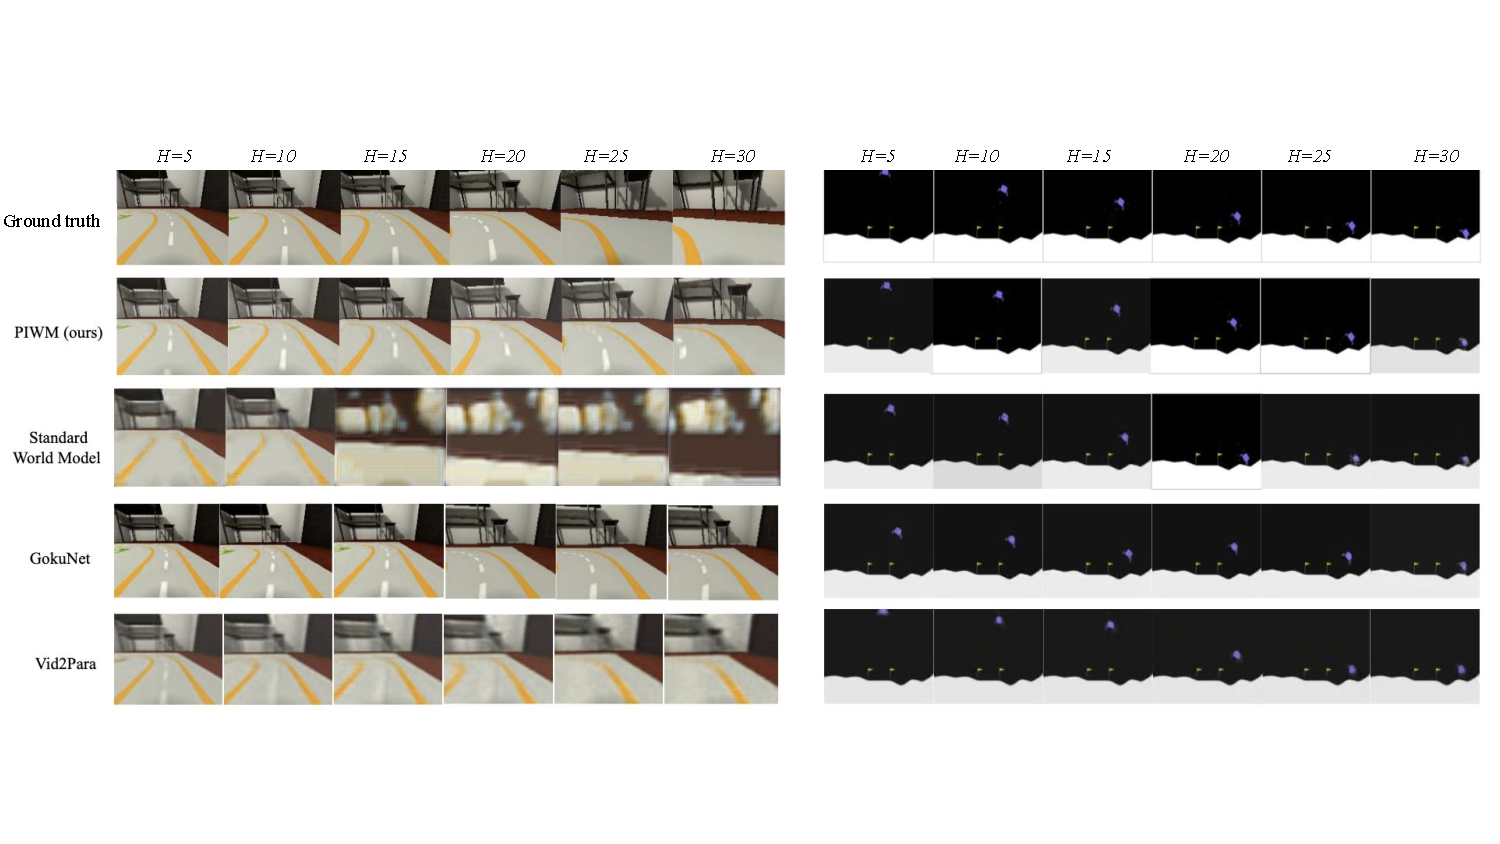
\includegraphics[width=1.9\columnwidth]{imgs/pred.pdf}
\caption{Qualitative comparison of 30-step trajectory rollouts under $\delta=5\%$.}	\label{fig:4}

 \end{figure*}

\paragraph{Continuous vs.\ discrete latent spaces.}
A key insight from these results is that {decoupling visual perception from physical state inference (the extrinsic approach) is a critical design choice for achieving robust, long-term prediction.} An important observation from our results is the different strengths exhibited by continuous and discrete latent parameterizations across the intrinsic and extrinsic settings. In the intrinsic (one-stage) architecture, the encoder must jointly learn visual abstractions and physically structured representations. This joint optimization benefits from the flexibility and smooth gradients of a continuous latent space, which can more easily adapt to the coupled visual–physical objectives. In contrast, the extrinsic (two-stage) architecture decouples visual encoding from physical interpretation. In this setting, the discrete latent space acts as a strong regularizer: the quantization suppresses visual noise, stabilizes the mapping to physical states, and improves generalization of the dynamics model. Consequently, the continuous variant performs better under the intrinsic setup, while the discrete variant achieves superior performance under the extrinsic setup. 

% This phenomenon reveals a key insight of our work: 

\textit{Takeaway:} the optimal latent parameterization depends on whether physical structure is learned jointly with perception or inferred from a pre-learned visual representation.
Furthermore, across both architectures, the quantized (discrete) latent space provides a powerful regularization effect, leading to more stable predictions than the continuous alternative, especially under noisy supervision.







 
\subsection{Physicality of Learned Representations}


Strong predictive performance should stem from accurate underlying states and dynamics. We validate this by evaluating the static encoding quality and the model's ability to recover the true physical parameters of the simulation.

As reported in the extended version~\cite{extended}, static encoding RMSE results show how accurately each model can infer the physical state from a single observation. The results strongly correlate with the predictive findings: the quantized extrinsic PIWM achieves the highest encoding accuracy, confirming that its superior representation is the foundation of its predictive power. The intrinsic continuous models, while competitive, exhibit higher encoding error, consistent with their weaker predictive performance.

Finally, we assess whether the dynamics model can learn the true physical parameters (e.g., car length, pole mass) within the learned latent space. As reported in Figure~\ref{fig:3}, PIWM successfully recovers the ground-truth parameters with low relative error across all environments. This provides direct evidence that our framework learns a genuinely interpretable representation that is not merely correlated with the physics --- but is structured in a physically grounded way. We emphasize that the DonkeyCar study is not designed to validate precise parameter recovery, since ground-truth physical parameters are unavailable, but rather to evaluate rollout stability and physical plausibility under approximate kinematic priors in a realistic robotic setting with visual sensing and control.









\section{Analysis and Discussion}\label{sec:dis}



Our experiment demonstrates that the extrinsic architecture with a discrete latent space is optimal for learning physically interpretable world models from weak supervision. This approach achieves superior prediction accuracy (Figure~\ref{fig:2}) by decoupling perception from physical state abstraction and leveraging quantization as a powerful regularizer against visual noise. The learned representations are not only predictive but also genuinely physically grounded, as evidenced by the model's ability to recover true system parameters (Figure~\ref{fig:3}) and generate qualitatively plausible visual rollouts that far exceed baseline performance (Figure~\ref{fig:4}). Crucially, the substantial gains in interpretability and prediction accuracy come at a minimal cost to downstream controller performance, as reported in the extended version~\cite{extended}. Across all variants and noise levels, action accuracy is largely preserved, confirming that physical interpretability does not degrade task-relevant visual fidelity. Notably, the extrinsic-discrete variant achieves the strongest balance between physical grounding and reconstruction quality for downstream control. DVBF performs poorly in our settings because its Gaussian latent space and amortized inference provide no physical inductive bias, causing the learned states to drift and quickly accumulate errors during multi-step rollouts. This makes DVBF unstable in visually rich or discontinuous dynamics environments, which explains its large performance gap relative to structured models such as PIWM.


While CartPole and Lunar Lander provide controlled benchmarks, DonkeyCar represents a real robotic platform with visual sensing, approximate physical modeling, and closed-loop control. Scaling PIWM to open-world CPS scenarios, such as multi-agent driving environments with richer state spaces, constitutes an important direction for future work. While our framework is effective, future work should also focus on scaling its representational capacity and enhancing its use of supervision. For complex, open-world scenarios like autonomous driving, our approach could be extended from predicting simple state vectors to building structured world representations, such as dynamic 3D occupancy grids, where physical priors can be applied to multiple agents. Furthermore, the rich temporal nature of weak supervision signals is currently underutilized. Future methods could process sequences of noisy supervisory signals using filtering or sequence modeling techniques to produce a more refined, temporally coherent learning target, thereby improving the model's robustness and accuracy. Also, the experiments in this work focus on Markovian dynamical systems, where transitions depend only on the most recent latent state and action. This setting aligns with the majority of prior work on world models and enables a clean evaluation of the proposed physically interpretable latent dynamics. Extending PIWM to non-Markovian or delayed-effect systems, where temporal dependencies span multiple steps, represents an interesting direction for future research. Evaluating such scenarios would require augmenting the dynamics model with additional memory mechanisms or explicitly modeling higher-order temporal dependencies. An important open question is whether the learned physically interpretable representations exhibit better compositional generalization and transfer properties than purely data-driven baselines, for example under unseen initial conditions, modified system parameters, or visual domain shifts. We expect physical grounding to provide a structural advantage in such scenarios, but systematic evaluation is left for future work. While PIWM currently requires a partially specified dynamics model, extending the framework to settings where the equation structure itself must be discovered, for example via symbolic regression or neural ODEs, represents a promising direction for future work.


 

\section{Related Work}\label{related}


\subsection{Trajectory Prediction}

% \noindent
% \textbf{Trajectory Prediction.}


Predicting trajectories is critical for safe planning and control~\cite[]{fridovich2020confidence}, but existing methods present trade-offs. While approaches like Hamilton-Jacobi (HJ) reachability offer formal guarantees~\cite[]{li2021prediction,nakamura2023online}, they are computationally expensive for online settings. Conversely, mainstream deep learning models are powerful but often rely on handcrafted scene representations~\cite[]{salzmann2020trajectron++} or high-precision maps~\cite[]{itkina2023interpretable, hsu2023interpretable}, and typically do not produce physically interpretable predictions~\cite[]{lu2024towards, lindemann2023conformal, ruchkin2022confidence}. In contrast, our approach learns directly from raw images with distribution-based weak supervision without requiring handcrafted inputs or goal conditioning.
% Predicting trajectories is critical for anticipating hazards like vehicle collisions, thus providing essential inputs to planning and control~\cite[]{fridovich2020confidence}. Methods such as Hamilton-Jacobi (HJ) reachability~\cite[]{li2021prediction,nakamura2023online} offer formal guarantees but require detailed dynamics knowledge and significant computations, limiting their scalability to high-dimensional online settings.  Online approaches, such as confidence-aware models~\cite[]{ruchkin2022confidence} and conformal prediction~\cite[]{lindemann2023conformal}, improve reliability but do not directly enhance physical interpretability. Deep architectures like Trajectron++~\cite[]{salzmann2020trajectron++} integrate scene graphs with conditional VAEs for multi-agent forecasting, though they still depend on handcrafted scene representations. To reduce the reliance on handcrafted features, Goal-based Neural Variational Agent (GNeVA)~\cite[]{lu2024towards} models spatial goal distributions using learnable priors, but it does not explicitly model interpretable physical variables, and thus offers limited insight into the physical dynamics underlying its predictions. Meanwhile, interpretable predictors like ISAP~\cite[]{itkina2023interpretable} use semantic information such as historical trajectories and high-precision maps, guided by human-aligned metrics~\cite[]{hsu2023interpretable}. In contrast, our approach learns directly from raw images with distribution-based weak supervision without requiring handcrafted inputs or goal conditioning.




\subsection{Representation Learning}


 % \noindent\textbf{Representation Learning.}

 
A central challenge in learning from high-dimensional sequences is creating compact and meaningful latent representations~\cite[]{shi2015convolutional,bai2018empirical}. While Variational Autoencoders (VAEs)~\cite[]{kingma2013auto} are foundational, their standard form learns unstructured latents. A significant line of research attempts to impose structure, either by encouraging disentanglement in continuous spaces with methods like \(\beta\)-VAE, FactorVAE, and TCVAE~\cite[]{higgins2017beta, kim2018disentangling, chen2018isolating}, or by enforcing causality~\cite[]{yang2021causalvae}. However, these methods often fall short of ensuring a direct correspondence with real-world physical states or require precisely labeled data. An alternative is to impose structure via discretization with Vector-Quantized VAEs (VQ-VAEs) and their extensions~\cite[]{van2017neural, razavi2019generating, xue2019supervised}. While effective, their application to physical prediction has been limited due to abstract latent codes and reliance on exact supervision. Even in robotic applications like DVQ-VAE that model structured systems, encoding external environmental factors remains a challenge~\cite[]{zhao2024decomposed}. GOKU-net constrains variables to plausible physical ranges but does not tie them to specific, interpretable quantities~\cite[]{linial_generative_2021}.

Other works incorporate structured priors to enhance learning. Object-centric world models like FOCUS~\cite[]{ferraro2023focus} and foundation world models~\cite{mao2024zero} improve efficiency by structuring latents around discrete entities. Models like SPARTAN~\cite []{lei2024spartan} provide outputs that are interpretable by construction but do not incorporate known physical dynamics or action-conditioned prediction. Priors can also be introduced as task-related rules in Bayesian neural networks~\cite[]{sam2024bayesian} or through human and self-supervision to guide abstraction~\cite[]{fu2021learning, wen2023any, konidaris2018skills, peng2024human, chen2022automated}. These approaches, however, often yield abstract representations that lack physical grounding without strong external priors. Closer to our work, Deep Variational Bayes Filters (DVBFs) extend VAEs with a latent dynamics module~\cite[]{karl2016deep}. Yet, without explicit physical supervision, they often fail to recover interpretable variables --- a limitation our work addresses by leveraging weak supervision.
% \textcolor{red}{
% \noindent\textbf{Representation Learning from introduction}
% Various architectures have been developed for sequence prediction from high-dimensional data. Convolutional LSTMs (ConvLSTMs), for instance, directly predict future observation sequences but can be complex and struggle with long-term temporal coherence~\cite[]{shi2015convolutional,bai2018empirical}. To create more compact and meaningful representations, a significant body of work has focused on improving the structure of latent spaces in Variational Autoencoders (VAEs). One major research thrust aims to learn disentangled representations in a continuous space, where individual latent dimensions correspond to independent data factors. Prominent methods in this area, including \(\beta\)-VAE, FactorVAE, and TCVAE, modify the VAE objective to enforce this separation~\cite[]{higgins2017beta, kim2018disentangling, chen2018isolating}. An alternative strategy imposes structure by discretizing the latent space. The Vector-Quantized VAE (VQ-VAE) achieves this by mapping representations to a learned, finite codebook, which can encourage the emergence of semantically meaningful latent codes~\cite[]{van2017neural}.}

% \noindent
% \textbf{Learning Latent Representations.}
% Latent representations enable neural networks to distill key features from high-dimensional data such as images, text, and audio~\cite[]{goodfellow2020generative,xie2016unsupervised,mao2024language,gatys2016image}. VAEs~\cite[]{kingma2013auto} learn compact latent spaces by encoding and reconstructing input data --- but lack interpretability and structure. Overcoming this, $\beta$-VAE~\cite[]{higgins2017beta} introduces a hyperparameter to encourage disentanglement, while CausalVAE~\cite[]{yang2021causalvae} further enforces causal relationships via a causal graph. However, both approaches often fail to ensure direct correspondence between latent variables and real-world physical states. They also require precisely labeled causal states, which can be difficult to obtain. 
% Another variant, GOKU-net~\cite[]{linial2021generative}, replaces the standard Gaussian prior with a learnable transformation that constrains the latent variables to lie within plausible physical ranges. However, these variables are not tied to specific physical quantities and thus are not interpretable.
% Unlike standard VAEs with continuous latents, VQ-VAEs~\cite[]{van2017neural} map inputs to discrete codebook entries. Their extensions, such as VQ-VAE-2~\cite[]{razavi2019generating} with hierarchical codebooks and S-VQ-VAE~\cite[]{xue2019supervised} with class-aligned supervision, improve reconstruction and feature alignment --- but have seen limited application to physical prediction due to abstract latents and reliance on exact supervision.
% % Variants such as DVQ-VAE~\cite[]{zhao2024decomposed}
% The closest robotic application is DVQ-VAE~\cite[]{zhao2024decomposed}, which employs multiple codebooks to model different parts of structured systems, such as using separate embeddings to represent robotic fingers and palms. However, such approaches still struggle to encode external environmental factors, limiting their physical interpretability.




 
% Structured priors are widespread in representation learning. For instance, task-related rules have been integrated into Bayesian neural networks~\cite[]{sam2024bayesian} to enhance performance. Similarly, object-centric world models like FOCUS~\cite[]{ferraro2023focus} and foundation world models~\cite[]{mao2024zero} structure latent spaces around discrete entities and interactions, improving learning efficiency and interpretability. 
% Other object-centric models like SPARTAN~\cite[]{lei2024spartan} provide semantically structured outputs interpretable by construction, but do not incorporate known physical dynamics or action-conditioned prediction.
% Human supervision can guide abstraction techniques~\cite[]{fu2021learning,wen2023any} to distill high-dimensional data into essential motion features to support policy learning~\cite[]{konidaris2018skills,peng2024human}. %  --- but usually rely on  and are difficult to map back to raw observations. 
% Self-supervision can learn minimal neural states~\cite[]{chen2022automated} with abstract representations that lack physical interpretability without external priors. Building on these ideas, we leverage task-relevant constraints in the form of dynamical equations and weak physical supervision to improve physical interpretability and accuracy. %, limiting their utility for interoperable trajectory prediction. 
% Deep variational Bayes filters (DVBF)~\cite[]{karl2016deep} extend VAE-based world models by introducing a latent dynamics module and an auxiliary physical value estimator. However, without explicit physical supervision, they often fail to recover interpretable variables, as we also observed in early experiments.


\subsection{World Models}


% \looseness=-1
% \noindent
% \textbf{World Models.}


Classical world models like Dreamer~\cite[]{hafner2020mastering} and DayDreamer~\cite[]{wu2023daydreamer} excel at learning from experience for policy learning, but their latent representations are typically uninterpretable~\cite[]{peper2025four}. Many approaches seek to improve physical grounding by incorporating priors, such as bounds on states and actions~\cite[]{tumu2023physics,sridhar2023guaranteed}, physics-aware loss functions~\cite[]{djeumou2023learn}, or kinematics-inspired layers~\cite[]{cui2020deep}. However, these methods are often designed for low-dimensional systems and do not scale well to learning from noisy, high-dimensional images. Other physics-informed methods leverage differential equations to stabilize learning~\cite[]{ZHONG2023115664,linial_generative_2021}, with frameworks like Phy-Taylor using Taylor monomials to structure the latent dynamics~\cite[]{mao_phy-taylor_2025}. Approaches like sparse identification and differentiable physics require access to the underlying state variables and are not designed to learn from raw visual inputs~\cite[]{yao2024marrying,BRUNTON2016710,de2018end}.

Recent advances have produced powerful but distinct world models. For instance, 3D occupancy-based models improve forecasting but their internal states are not explicitly aligned with physical variables~\cite[]{zheng2024occworld,min2023uniworld,yan2024renderworld,zuo2024gaussianworld}. Concurrently, neuro-symbolic models enhance generalization but require predefined symbolic inputs not available from raw sensor data~\cite[]{balloch2023neuro,liang2024visualpredicator}. Our approach is distinct from these paradigms as it learns physically interpretable representations directly from images using weak supervision. This also contrasts with the most closely related work, Vid2Param~\cite[]{asenov2019vid2param}, which requires full supervision and struggles with dynamics prediction.






% \section{Limitations}\label{sec:limit}

\section{Conclusion}\label{sec:conclusion}
We presented the Physically Interpretable World Model, a framework that learns physically-grounded latent representations from images using only weak distributional supervision. Our systematic evaluation demonstrates that an extrinsic architecture with a discrete latent space yields accurate and robust predictions and successfully recovers the system's true physical parameters. This work not only provides direct evidence of a physically interpretable model --- but also offers a practical path toward more trustworthy and reliable cyber-physical systems with generative predictors. 


\section*{Acknowledge}\label{sec:ack}
 
The authors thank Liam (Cade) McGlothlin and Vedansh Maheshwari for their help in exploring interpretable world models. The authors also appreciate the feedback of the anonymous reviewers. 

This material is based upon work supported by the U.S. National Science Foundation (NSF) under Grant Numbers CNS 2513076 and CCF 2403616. Any opinions, findings, and conclusions or recommendations expressed in this material are those of the authors and do not necessarily reflect the views of the NSF.

% \begin{acks}
% To Robert, for the bagels and explaining CMYK and color spaces.
% \end{acks}

\newpage

\bibliographystyle{ACM-Reference-Format}
\bibliography{sample-base}

\clearpage

\newpage

\appendix
\section*{Appendix}

\textbf{Model Architecture and Training Details.} This appendix provides detailed implementation specifications for the Physically
Interpretable World Model (PIWM) and its four instantiations:
intrinsic--continuous, intrinsic--discrete, extrinsic--continuous, and
extrinsic--discrete. All variants follow the unified formulation introduced in
Section~\ref{sec:architecture}, operating on the same dataset, the same weak
supervision mechanism, and the same training objective.

\subsubsection*{A. Vision Encoders and Decoders}

All variants share the same convolutional vision encoder $\mathcal{E}_v$ and
decoder $\mathcal{D}_v$. The encoder contains two convolutional layers with ReLU
activations and maps each observation $y_t$ to an intermediate latent vector
$z_t \in \mathbb{R}^{64}$. The decoder $\mathcal{D}_v$ mirrors this structure
and reconstructs an image $\hat{y}_{t+2}$ from a latent representation.  
Continuous variants use a standard $\beta$-VAE objective on $z_t$ with
$\beta = 1$, while discrete variants apply a VQ-VAE quantization layer with a
codebook of 512 learnable embeddings of dimension 64, trained using a
commitment weight of $\beta = 0.25$.

\subsubsection*{B. Physical Encoder $\mathcal{E}_p$}

In extrinsic architectures, the interpretable latent state is produced by a
physical encoder $\mathcal{E}_p$ applied to the intermediate visual latent:
\[
z^*_t = \mathcal{E}_p(z_t).
\]
This module is implemented as a Transformer encoder with two layers, four
attention heads per layer, a model dimension of 128, and a feedforward width of
512. Mean pooling across tokens is followed by a linear projection to produce
the final interpretable state $z^*_t$. The physical encoder is trained entirely
via the interpretability loss $\mathcal{L}_{\text{interp}}(z^*_t, \Xi_t)$.

\subsubsection*{C. Intrinsic Representation Learning}

Intrinsic variants produce the interpretable latent state directly from images,
\[
z^*_t = \mathcal{E}(y_t),
\]
without an intermediate latent or a separate physical encoder.  
For intrinsic--continuous models, $\mathcal{E}$ outputs the parameters of a
Gaussian distribution over the latent $z^*_t \in \mathbb{R}^{64}$, where a fixed
subset of dimensions corresponds to the physical component $z^{*}_{p,t}$.  
The loss combines reconstruction, interpretability alignment, and KL
regularization following the $\beta$-VAE formulation.

For intrinsic--discrete models, a VQ-VAE codebook of 512 embeddings is used.
Each embedding vector is partitioned as
$\mathbf{e}_k = [\mathbf{e}^{p}_k,\, \mathbf{e}^{v}_k]$, matching the structure
in Section~\ref{sec:architecture}. The interpretable state is computed from the
physical portion of the selected codebook entry, and the interpretability loss is
applied directly to this physical component.

\subsubsection*{D. Dynamics Model}

All variants share the same structured second-order latent dynamics model
described in Section~\ref{sec:architecture}:
\[
z^{*}_{t+2} = \phi_\theta(z^{*}_{t},\, z^{*}_{t+1},\, a_t).
\]
The functional form of $\phi_\theta$ is derived from the physics of each
environment (e.g., kinematics), with only the parameters $\theta$ being
learnable. Depending on the environment, $\phi_\theta$ contains between 4 and 10
unknown physical parameters. A two-step initialization window
$(z^*_t, z^*_{t+1})$ provides the required derivative information for
prediction, such as implicit velocities.  

At each time step, weak supervision consists of a set of $L = 50$ proxy samples
$\Xi_t = \{\xi^{(l)}_t\}$ drawn from the unknown distribution $p(x_t)$. The
dynamics loss is computed as
\[
\mathcal{L}_{\text{dyn}} = 
\| z^{*}_{t+H} - \hat{\mu}_{\xi_{t+H}} \|_2^2,
\]
where $\hat{\mu}_{\xi_t}$ is the empirical sample mean of $\Xi_t$.

\subsubsection*{E. Loss Functions}

All variants are trained using the unified objective:
\[
\mathcal{L} =
\mathcal{L}_{\text{rec}}
+ \lambda_1 \mathcal{L}_{\text{interp}}
+ \lambda_2 \mathcal{L}_{\text{dyn}}
+ \lambda_3 \mathcal{L}_{\text{reg}}.
\]
The reconstruction loss is mean squared error in image space:
\[
\mathcal{L}_{\text{rec}}
= \| \mathcal{D}_v(z_{t+2}) - y_{t+2} \|_2^2.
\]
The interpretability loss uses the weak supervision samples:
\[
\mathcal{L}_{\text{interp}}
= \| z^{*}_{p,t} - \hat{\mu}_{\xi_t} \|_2^2.
\]

Continuous variants use KL regularization consistent with the $\beta$-VAE
formulation, whereas discrete variants use VQ-VAE codebook and commitment
losses, matching the structure defined in Section~\ref{sec:architecture}.

\subsubsection*{F. Training Setup}

All models are trained using the Adam optimizer with batch size 32. Continuous
variants use an initial learning rate of $10^{-4}$, and discrete variants use
$10^{-3}$ due to the stochasticity introduced by quantization. A cosine decay
schedule with 5 warmup epochs is applied. Training proceeds for up to 200
epochs, with early stopping after 20 epochs of no validation improvement.  
Gradient norms are clipped at 1.0 for stability.  
Evaluation uses 30-step prediction rollouts in latent space, decoding to images
only when needed.

Weak supervision is applied consistently across noise settings
$\delta \in \{0\%, 5\%, 10\%\}$.

\subsubsection*{G. Summary of Differences Between Variants}

Intrinsic models produce $z^{*}_t$ directly from observations, whereas extrinsic
models obtain $z^{*}_t$ through the composition
$z^*_t = \mathcal{E}_p(\mathcal{E}_v(y_t))$.  
Continuous variants use Gaussian latent parameterizations, and discrete variants
use a VQ-VAE codebook with 512 entries.  
Across all variants, the interpretable component of the latent occupies a fixed
subset of dimensions. All models share identical dynamics functions
$\phi_\theta$ and training losses.

\subsubsection*{H. Architectural Details in Text}

All models use a shared two-layer CNN vision encoder and decoder producing a
64-dimensional latent space. Continuous variants use Gaussian latents with a KL
penalty, while discrete variants use a 512-entry VQ-VAE codebook trained with a
commitment weight of $\beta=0.25$.  
Extrinsic variants include a two-layer Transformer physical encoder with model
dimension 128. Intrinsic variants instead embed the physical portion directly
into $z^*_t$.  
The dynamics model learns between 4 and 10 environment-specific parameters using
50 weak supervision samples per time step.

\subsubsection*{I. Training Hyperparameters in Text}

All experiments use batch size 32, cosine learning-rate decay with 5 warmup
epochs, a maximum of 200 epochs with patience 20, and gradient clipping at
1.0. Rollouts span 30 steps in latent space. All environments use the same
60{,}000-trajectory dataset and weak supervision noise levels
$\delta \in \{0\%, 5\%, 10\%\}$.

\begin{figure*}[!htbp]
    \centering
    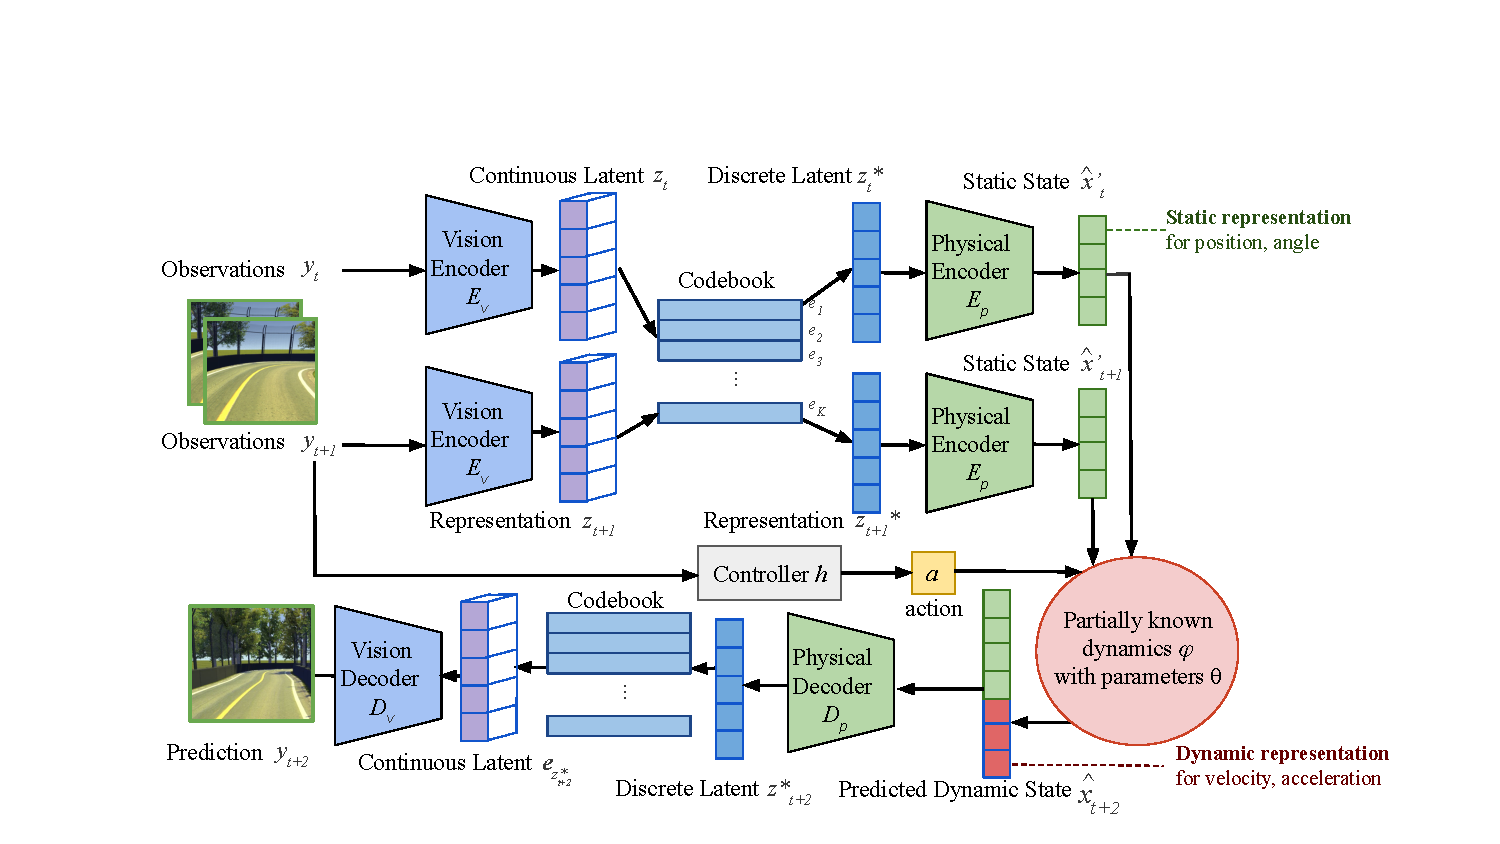
\includegraphics[width=1.95\columnwidth]{imgs/vq.pdf}
\caption{
\textbf{Extrinsic–discrete PIWM architecture.}
The vision encoder $\mathcal{E}_v$ produces latents $z_t$, which are quantized
to $z_t^{*}$ and mapped to physical states by $\mathcal{E}_p$. The dynamics
model $\phi_\theta$ predicts $\hat{x}_{t+2}$ from two physical states and
action $a_t$, and the decoders $\mathcal{D}_p$ and $\mathcal{D}_v$ reconstruct
the predicted observation.
}
    \label{fig:extrinsic-vq-appendix}
\end{figure*}


\begin{figure}[h]
	\centering         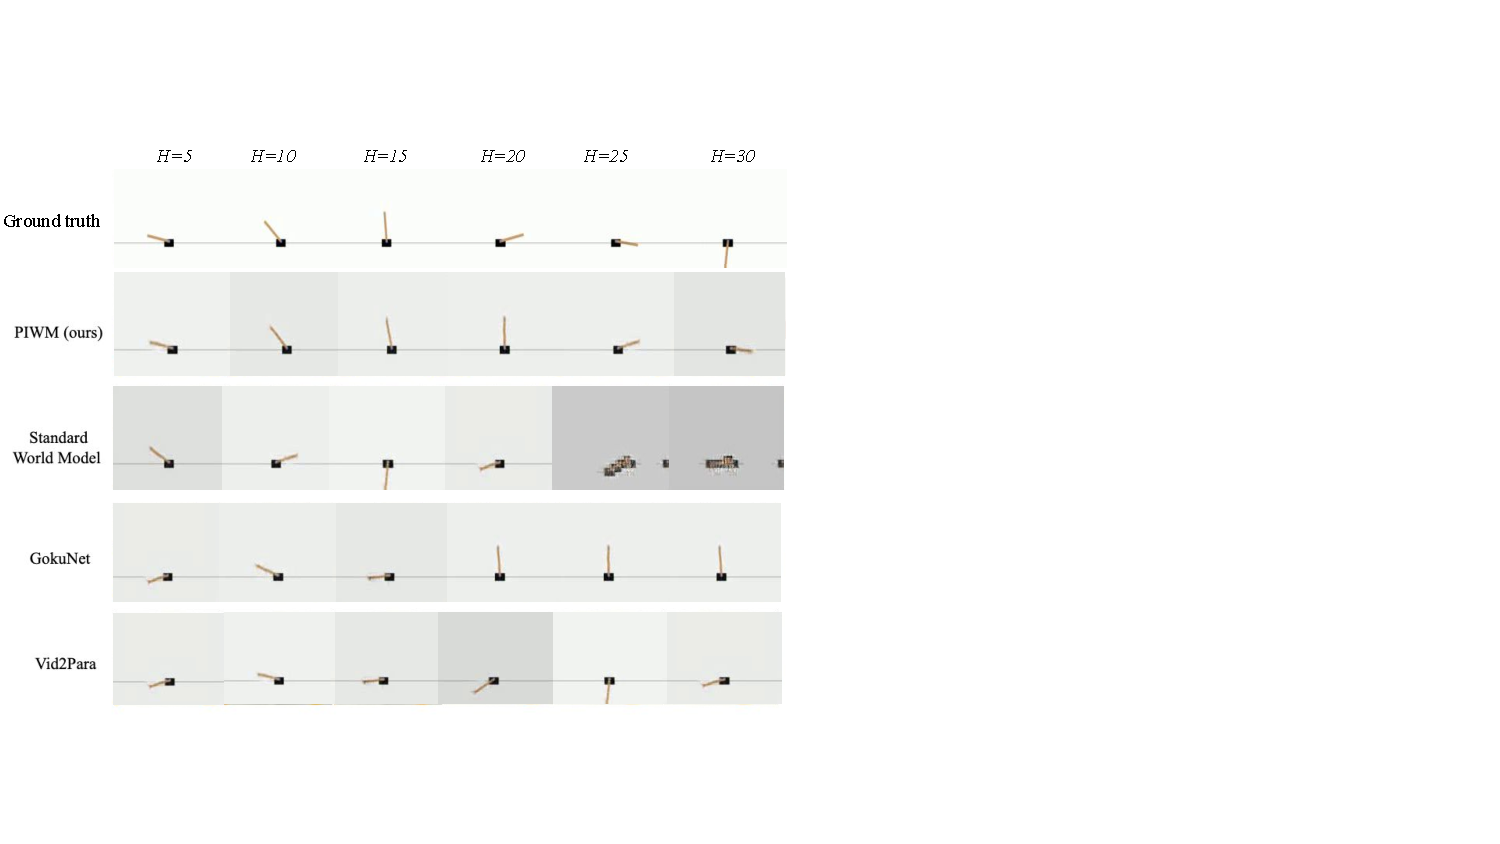
\includegraphics[width=0.95\columnwidth]{imgs/cartviz.pdf}
\caption{Qualitative comparison of 30-step trajectory rollouts under $\delta=5\%$ of Cart Pole.}	\label{fig:cartviz}
 \end{figure}





\textbf{Architecture for the Extrinsic-Discrete Variant}. 
This section provides an expanded diagram of the \emph{extrinsic-discrete}
variant of PIWM, which is used in our experiments.  
Unlike intrinsic variants, the extrinsic pipeline decouples visual perception
from physical interpretation: a VQ-based vision autoencoder first produces a
discrete latent representation, after which a dedicated physical encoder
extracts the interpretable physical state.  
This figure visualizes the complete data flow from raw observations to discrete
latents, physical state estimation, structured dynamics prediction, and
final reconstruction.


\textbf{Controller Performance on Reconstructions.}
To assess whether PIWM variants preserve task-relevant visual information, we
evaluate how well reconstructed observations $\hat{y}_{t}$ support action
prediction when passed through the environment’s original controller $h$.  
Table~\ref{tab:2} summarizes controller performance (action RMSE
for Donkey Car; action accuracy for Lunar Lander and CartPole) for all four
architectural variants and all supervision noise levels.  
These results provide a complementary diagnostic showing how the different
latent designs affect the quality of reconstructed observations for downstream
control.


\begin{table}[ht!]
\centering
\caption{Controller Performance on Reconstructed Observations Across All Variants and Noise Levels}
\label{tab:2}
\tiny % Using a smaller font size for this dense table
\begin{tabular}{@{}ll l ccc@{}}
\toprule
\multirow{2}{*}{\textbf{Case}} & \multirow{2}{*}{\textbf{Input Type}} & \multirow{2}{*}{\textbf{Latent Space}} & \multicolumn{3}{c}{\textbf{Supervision Noise Level ($\delta$)}} \\
\cmidrule(l){4-6}
& & & \textbf{0\%} & \textbf{5\%} & \textbf{10\%} \\
\midrule
\multirow{5}{*}{\shortstack{Donkey Car \\ (Action RMSE $\downarrow$)}}
& \multirow{2}{*}{One-Stage (Intrinsic)} & Continuous & $0.12 \pm 0.04$ & $0.13 \pm 0.04$ & $0.15 \pm 0.05$ \\
& & Discrete & $0.21 \pm 0.15$ & $0.29 \pm 0.16$ & $0.32 \pm 0.20$ \\
\cmidrule(l){2-6}
& \multirow{2}{*}{Two-Stage (Extrinsic)} & Continuous & $0.15 \pm 0.05$ & $0.16 \pm 0.05$ & $0.22 \pm 0.06$ \\
& & Discrete & $0.15 \pm 0.04$ & $0.17 \pm 0.05$ & $0.19 \pm 0.05$ \\
\midrule
\multirow{5}{*}{\shortstack{Lunar Lander \\ (Action Acc. $\uparrow$)}}
& \multirow{2}{*}{One-Stage (Intrinsic)} & Continuous & $93.0\% \pm 1.8\%$ & $90.5\% \pm 2.0\%$ & $87.1\% \pm 2.2\%$ \\
& & Discrete & $85.5\% \pm 2.5\%$ & $82.1\% \pm 2.8\%$ & $78.3\% \pm 3.1\%$ \\
\cmidrule(l){2-6}
& \multirow{2}{*}{Two-Stage (Extrinsic)} & Continuous & $86.2\% \pm 2.4\%$ & $83.5\% \pm 2.6\%$ & $80.0\% \pm 2.9\%$ \\
& & Discrete & $91.5\% \pm 2.1\%$ & $88.6\% \pm 2.3\%$ & $84.5\% \pm 2.5\%$ \\
\midrule
\multirow{5}{*}{\shortstack{Cart Pole \\ (Action Acc. $\uparrow$)}}
& \multirow{2}{*}{One-Stage (Intrinsic)} & Continuous & $98.0\% \pm 1.0\%$ & $96.5\% \pm 1.2\%$ & $94.0\% \pm 1.5\%$ \\
& & Discrete & $95.0\% \pm 1.6\%$ & $91.5\% \pm 2.0\%$ & $87.2\% \pm 2.5\%$ \\
\cmidrule(l){2-6}
& \multirow{2}{*}{Two-Stage (Extrinsic)} & Continuous & $95.5\% \pm 1.5\%$ & $92.0\% \pm 1.8\%$ & $88.0\% \pm 2.2\%$ \\
& & Discrete & $97.2\% \pm 1.1\%$ & $95.0\% \pm 1.4\%$ & $92.5\% \pm 1.8\%$ \\
\bottomrule
\end{tabular}
\end{table}




% ============================================================
% Algorithm: Cart Pole Dynamics
% ============================================================

\newpage


\begin{algorithm}[h]
\caption{Dynamics of Cart Pole}
\label{alg:pendulum_dynamics}
\begin{algorithmic}[1]
\Require Current state $z = [x, \dot{x}, \theta, \dot{\theta}]$, action $a$
\Ensure  Updated state $z_{\text{new}} = [x_{\text{new}}, \dot{x}_{\text{new}}, \theta_{\text{new}}, \dot{\theta}_{\text{new}}]$

\State \textbf{// Extract State Variables}
\State $x,\ \dot{x},\ \theta,\ \dot{\theta}
       \gets z[:,0],\ z[:,1],\ z[:,2],\ z[:,3]$

\State \textbf{// Convert Action to Force}
\State $F \gets \text{force\_mag} \times (2 \cdot a - 1)$

\State \textbf{// Compute Trigonometric Values}
\State $\cos\theta \gets \text{costheta},\quad \sin\theta \gets \text{sintheta}$

\State \textbf{// Compute Intermediate Variable}
\State $\text{temp} \gets
       \dfrac{F + m_p \cdot l \cdot \dot{\theta}^2 \cdot \sin\theta}
             {m_p + m_c}$

\State \textbf{// Calculate Angular Acceleration}
\State $\ddot{\theta} \gets
       \dfrac{g \cdot \sin\theta - \cos\theta \cdot \text{temp}}
             {l \cdot \left(\dfrac{4}{3}
              - \dfrac{m_p \cdot \cos^2\!\theta}{m_p + m_c}\right)}$

\State \textbf{// Calculate Linear Acceleration}
\State $\ddot{x} \gets \text{temp}
       - \dfrac{m_p \cdot l \cdot \ddot{\theta} \cdot \cos\theta}{m_p + m_c}$

\State \textbf{// Update State Variables}
\State $x_{\text{new}}         \gets x         + \tau \cdot \dot{x}$
\State $\dot{x}_{\text{new}}   \gets \dot{x}   + \tau \cdot \ddot{x}$
\State $\theta_{\text{new}}    \gets \theta     + \tau \cdot \dot{\theta}$
\State $\dot{\theta}_{\text{new}} \gets \dot{\theta} + \tau \cdot \ddot{\theta}$

\State \Return
       $z_{\text{new}} \gets
       [x_{\text{new}},\ \dot{x}_{\text{new}},\
        \theta_{\text{new}},\ \dot{\theta}_{\text{new}}]$
\end{algorithmic}
\end{algorithm}


% ============================================================
% Algorithm: Lunar Lander Dynamics
% ============================================================

\newpage



\begin{algorithm}[h]
\caption{Dynamics of Lunar Lander}
\label{alg:lunar_lander_dynamics}
\begin{algorithmic}[1]
\Require Current states
         $\mathbf{s} = [x, y, \dot{x}, \dot{y}, \theta, \dot{\theta}]$,
         actions $\mathbf{a}$
         \textit{(0: do nothing, 1: fire left, 2: fire main, 3: fire right)}
\Ensure  Updated states
         $\mathbf{s}_{\text{new}} =
         [x_{\text{new}}, y_{\text{new}},
          \dot{x}_{\text{new}}, \dot{y}_{\text{new}},
          \theta_{\text{new}}, \dot{\theta}_{\text{new}}]$

\State \textbf{// Unpack State Variables}
\State $x \gets \mathbf{s}[:,0],\quad y \gets \mathbf{s}[:,1]$
\State $\dot{x} \gets \mathbf{s}[:,2],\quad \dot{y} \gets \mathbf{s}[:,3]$
\State $\theta \gets \mathbf{s}[:,4],\quad \dot{\theta} \gets \mathbf{s}[:,5]$

\State \textbf{// Calculate Engine Direction and Dispersion}
\State $\text{tip}  \gets [\sin\theta,\ \cos\theta]$
\State $\text{side} \gets [-\cos\theta,\ \sin\theta]$

\State \textbf{// Process Actions}
\State $\text{fire\_main}  \gets (\mathbf{a} == 2)$
\State $\text{fire\_left}  \gets (\mathbf{a} == 1)$
\State $\text{fire\_right} \gets (\mathbf{a} == 3)$

\State \textbf{// Compute Main Engine Thrust}
\State $m_{\text{power}} \gets \text{fire\_main}$
\State $\dot{x} \gets \dot{x}
       - \text{tip}[:,0] \cdot \text{main\_power}
         \cdot m_{\text{power}} \;/\; \text{FPS}$
\State $\dot{y} \gets \dot{y}
       + \text{tip}[:,1] \cdot \text{main\_power}
         \cdot m_{\text{power}} \;/\; \text{FPS}$

\State \textbf{// Compute Side Engine Thrust}
\State $s_{\text{power}}  \gets \text{fire\_left} + \text{fire\_right}$
\State $\text{direction}  \gets \text{fire\_right} - \text{fire\_left}$
\State $\dot{x} \gets \dot{x}
       + \text{side}[:,0] \cdot \text{side\_power}
         \cdot s_{\text{power}} \cdot \text{direction} \;/\; \text{FPS}$
\State $\dot{\theta} \gets \dot{\theta}
       + \text{side\_power} \cdot s_{\text{power}}
         \cdot \text{direction} \;/\; \text{FPS}$

\State \textbf{// Update Position and Angle}
\State $x      \gets x      + \dot{x}      / \text{FPS}$
\State $y      \gets y      + \dot{y}      / \text{FPS}$
\State $\theta \gets \theta + \dot{\theta} / \text{FPS}$

\State \Return
       $\mathbf{s}_{\text{new}} \gets
       [x,\ y,\ \dot{x},\ \dot{y},\ \theta,\ \dot{\theta}]$
\end{algorithmic}
\end{algorithm}


% ============================================================
% Algorithm: Bicycle Model Dynamics
% ============================================================
\begin{algorithm}[h]
\caption{Dynamics of Bicycle Model}
\label{alg:bicycle_dynamics}
\begin{algorithmic}[1]
\Require Current state $s = [x, y, \theta, v]$,
         action $a = [\delta,\, a_{\text{acc}}]$
\Ensure  Updated state
         $s_{\text{new}} =
         [x_{\text{new}}, y_{\text{new}}, \theta_{\text{new}}, v_{\text{new}}]$

\State \textbf{// Extract State Variables}
\State $x,\ y,\ \theta,\ v
       \gets s[:,0],\ s[:,1],\ s[:,2],\ s[:,3]$

\State \textbf{// Extract Action Variables}
\State $\delta,\ a_{\text{acc}} \gets a[:,0],\ a[:,1]$

\State \textbf{// Update State Variables}
\State $x_{\text{new}}      \gets x      + v \cdot \cos(\theta) \cdot \tau$
\State $y_{\text{new}}      \gets y      + v \cdot \sin(\theta) \cdot \tau$
\State $\theta_{\text{new}} \gets \theta + \dfrac{v}{L} \cdot \tan(\delta) \cdot \tau$
\State $v_{\text{new}}      \gets v      + a_{\text{acc}} \cdot \tau$

\State \Return
       $s_{\text{new}} \gets
       [x_{\text{new}},\ y_{\text{new}},\
        \theta_{\text{new}},\ v_{\text{new}}]$
\end{algorithmic}
\end{algorithm}






\begin{table*}[ht!]
\centering
\caption{
\textbf{Static state encoding error under weak supervision.}
For each environment and model variant, we report the mean~$\pm$~std of 
(1) MSE between the predicted static latent $z^{*}_{p}$ and the empirical mean 
of the weak-supervision samples, and 
(2) KL divergence for continuous variants.  
Columns correspond to different supervision noise levels $\delta$.
Lower values indicate better alignment between latent representations and 
static physical state variables (e.g., position, angle).
}
\label{tab:static_rmse_all_noise}
\footnotesize % Use \small or \footnotesize to adjust the font size
\begin{tabular}{@{}llcccccc@{}}
\toprule
\multirow{2}{*}{\textbf{Case}} & \multirow{2}{*}{\textbf{Model}} & \multicolumn{2}{c}{\textbf{$\delta = 0\%$}} & \multicolumn{2}{c}{\textbf{$\delta = 5\%$}} & \multicolumn{2}{c}{\textbf{$\delta = 10\%$}} \\
\cmidrule(lr){3-4} \cmidrule(lr){5-6} \cmidrule(lr){7-8}
 &  & \textbf{MSE} & \textbf{KL} & \textbf{MSE} & \textbf{KL} & \textbf{MSE} & \textbf{KL} \\ \midrule
\multirow{4}{*}{Donkey Car} & Intrinsic (Cont.) & $0.13 \pm 0.05$ & $0.45 \pm 0.06$ & $0.16 \pm 0.06$ & $0.52 \pm 0.07$ & $0.20 \pm 0.07$ & $0.58 \pm 0.08$ \\
 & Intrinsic (Disc.) & $0.18 \pm 0.04$ & $0.42 \pm 0.05$ & $0.21 \pm 0.05$ & $0.55 \pm 0.06$ & $0.22 \pm 0.06$ & $0.64 \pm 0.07$ \\
 & Extrinsic (Cont.) & $0.11 \pm 0.05$ & $0.24 \pm 0.04$ & $0.15 \pm 0.04$ & $0.28 \pm 0.05$ & $0.16 \pm 0.05$ & $0.33 \pm 0.06$ \\
 & \textbf{Extrinsic (Disc.)} & {$0.03 \pm 0.02$} & $0.19 \pm 0.03$ & {$0.05 \pm 0.03$} & $0.23 \pm 0.04$ & {$0.06 \pm 0.04$} & $0.28 \pm 0.05$ \\ \midrule
\multirow{4}{*}{Lunar Lander} & Intrinsic (Cont.) & $0.07 \pm 0.05$ & $0.56 \pm 0.26$ & $0.08 \pm 0.15$ & {$0.58 \pm 0.37$} & $0.21 \pm 0.07$ & $0.77 \pm 0.38$ \\
 & Intrinsic (Disc.) & $0.06 \pm 0.04$ & $0.44 \pm 0.11$ & $0.03 \pm 0.05$ & $0.53 \pm 0.12$ & $0.16 \pm 0.06$ & $0.64 \pm 0.17$ \\
 & Extrinsic (Cont.) & $0.11 \pm 0.07$ & $0.33 \pm 0.14$ & $0.14 \pm 0.04$ & $0.39 \pm 0.16$ & $0.15 \pm 0.05$ & $0.45 \pm 0.26$ \\
 & \textbf{Extrinsic (Disc.)} & \textbf{$0.03 \pm 0.02$} & $0.24 \pm 0.14$ & \textbf{$0.09 \pm 0.03$} & $0.29 \pm 0.11$ & \textbf{$0.12 \pm 0.04$} & $0.35 \pm 0.23$ \\ \bottomrule
\end{tabular}
\end{table*}


% ----------------------------------

% \appendix
% \section*{Appendix}

% \subsection*{Model Architecture and Training Details}

% This appendix provides additional implementation details for the Physically
% Interpretable World Model (PIWM) and the four model variants evaluated in the
% experiments: intrinsic--continuous, intrinsic--discrete, extrinsic--continuous,
% and extrinsic--discrete. All models share the same dataset, the same weak
% supervision mechanism, and the same evaluation protocol described in
% Section~4.

% \subsubsection*{A. Vision Encoders and Decoders}

% All variants use the same convolutional vision encoder $E_v$ and decoder $D_v$.
% The encoder consists of two convolutional layers with ReLU activations and
% projects each input image into a 64-dimensional latent vector 
% $z_t \in \mathbb{R}^{64}$. The decoder mirrors this structure and reconstructs
% the next image $\hat{y}_{t+2}$ from the predicted latent $z_{t+2}$. Continuous
% variants employ a standard $\beta$-VAE formulation with $\beta=1$, while
% discrete variants use a VQ-VAE quantization layer with a 512-entry codebook,
% each embedding being 64-dimensional and trained with a commitment loss weight of
% $\beta=0.25$.

% \subsubsection*{B. Physical Encoder $E_p$}

% For extrinsic variants, the mapping from visual latents to physical latents
% is performed by a dedicated physical encoder $E_p$. This network is a
% lightweight Transformer encoder with two layers, each containing four attention
% heads, a model dimension of 128, and a feedforward network width of 512. After
% Transformer processing, mean pooling is applied and followed by a linear
% projection to obtain $z^{*}_t$. This module is trained exclusively through weak
% supervision via $L_{\text{interp}}$.

% \subsubsection*{C. Intrinsic Representation Learning}

% In intrinsic variants, the physical latent is produced directly from images,
% $z^{*}_t = E(y_t)$, without using a separate $E_p$. For intrinsic--continuous,
% the latent space has dimension 64, and the first 2 dimensions are assigned to
% physical state variables while the remaining 62 dimensions correspond to visual
% factors. For intrinsic--discrete, the VQ codebook contains 512 embeddings of
% dimension 64, and each embedding is partitioned in the same manner: the first 2
% dimensions correspond to physical components, with the remaining 62 capturing
% visual variations.

% \subsubsection*{D. Dynamics Model}

% All four variants use the same second-order latent dynamics model,
% \[
% z^{*}_{t+2} = \phi_\theta(z^{*}_{t}, z^{*}_{t+1}, a_t),
% \]
% where the functional form follows the physics equations of the environment.
% Across different environments, the number of learnable physical parameters
% ranges from 4 to 10. A two-step initialization window $(z^{*}_t, z^{*}_{t+1})$
% provides the implicit velocity and derivative information needed for prediction.
% Weak supervision provides 50 proxy samples at every time step, and these are
% used to compute the dynamics loss 
% $L_{\text{dyn}} = \|z^{*}_{t+k} - \mu_{\Xi_{t+k}}\|^2_2$.

% \subsubsection*{E. Loss Functions}

% The training objective is
% \[
% L = L_{\text{rec}} + \lambda_1 L_{\text{interp}}
%     + \lambda_2 L_{\text{dyn}} + \lambda_3 L_{\text{reg}}.
% \]
% The reconstruction loss uses mean-squared error,
% $L_{\text{rec}} = \|D_v(z_{t+2}) - y_{t+2}\|^2_2$. The interpretability loss,
% applied using the 50 weak-supervision samples at each time step, is
% $L_{\text{interp}} = \|z^{*}_{p,t} - \mu_{\Xi_t}\|^2_2$. Continuous variants use
% a KL penalty with weight $\beta=1$ for regularization, whereas discrete variants
% use a VQ commitment loss with weight $\beta=0.25$.

% \subsubsection*{F. Training Setup}

% Across all variants, training uses the Adam optimizer with a batch size of 32.
% Continuous variants use an initial learning rate of $10^{-4}$, whereas discrete
% variants use $10^{-3}$ due to the additional stochasticity introduced by
% quantization. The learning rate follows a cosine decay schedule with a warmup
% period of 5 epochs. Training proceeds for at most 200 epochs, with early
% stopping based on a patience threshold of 20 validation epochs. Gradient norms
% are clipped at 1.0 to maintain stability. For evaluation, models perform
% 30-step latent rollouts, decoding only when reconstruction metrics are needed.
% Weak supervision is applied consistently across all noise levels
% $\delta \in \{0\%, 5\%, 10\%\}$.

% \subsubsection*{G. Summary of Differences Between Variants}

% Intrinsic and extrinsic variants differ in whether $z^{*}$ is produced
% directly (intrinsic) or through an additional physical encoder (extrinsic).
% Continuous and discrete variants differ in whether the latent representation is
% a 64-dimensional Gaussian vector (continuous) or a 512-entry codebook with
% 64-dimensional embeddings (discrete). In all cases, the physical state occupies
% the first 2 latent dimensions. The core dynamics learning procedure and training
% pipeline remain identical across all variants.

% \subsubsection*{H. Architectural Details in Text}

% All models share the same 64-dimensional latent visual space and two-layer CNN
% encoder/decoder backbone. Continuous variants represent latents through a
% 64-dimensional Gaussian vector with a standard VAE KL penalty. Discrete variants
% replace this with a VQ-VAE codebook containing 512 embeddings of dimension 64,
% trained with a commitment cost of $\beta = 0.25$. Extrinsic variants include an
% additional physical encoder with two Transformer layers, each having four
% attention heads, a model dimension of 128, and feedforward layers of width 512.
% The intrinsic variants instead embed the physical dimensions directly within the
% encoder output. All dynamics models estimate between 4 and 10 parameters
% depending on the environment, and all use 50 weak-supervision samples per
% timestep to compute both interpretability and dynamics losses.

% \subsubsection*{I. Training Hyperparameters in Text}

% Training is conducted with a batch size of 32 for all variants. Continuous
% models begin with a learning rate of $10^{-4}$, while discrete models begin at
% $10^{-3}$. A cosine learning-rate schedule with 5 warmup epochs is applied
% throughout training. Up to 200 epochs are allowed, although early stopping with
% patience 20 generally halts training earlier. Gradient clipping at a global norm
% of 1.0 is used to prevent instability. For evaluation, each model performs
% 30-step prediction rollouts in latent space. All experiments use the same
% 60,000-trajectory dataset and the same weak supervision noise settings
% $\delta \in \{0\%, 5\%, 10\%\}$.






% \newpage

% \appendix

% \section*{Appendix}




% \subsection*{A. Training  Algorithms}


% The training procedures for the ablation and proposed models are summarized in Algorithm~\ref{alg:ablated_train} and Algorithm~\ref{alg:piwm_train}, respectively.

% For the PIWM model (Algorithm~\ref{alg:piwm_train}), observations are first encoded into discrete latent representations using a Vision VQ-VAE module. These discrete latents are further mapped into interpretable physical states via a physical encoder $\mathcal{E}_p$. The dynamics model $\phi_\theta$ predicts the future physical state based on the current and next physical states. The predicted physical state is decoded back into the latent space and finally reconstructed into the future observation. The loss is computed similarly, with both reconstruction and weak supervision terms.

% For the ablation model (Algorithm~\ref{alg:ablated_train}), consecutive observations are first encoded using the encoder $\mathcal{E}$ into latent variables. The dynamics model $\phi_\theta$ predicts the future latent state by taking as input the latent representations from two consecutive frames. The decoder $\mathcal{D}$ reconstructs the observation at the future time step, and a reconstruction loss is computed. In addition, a weak supervision loss is applied to regularize the encoded latents based on interval labels.



% The main difference between the ablation and proposed models lies in the latent structure and dynamics modeling: the ablation model operates directly in the visual latent space, while the proposed model enforces a structured, interpretable physical latent space for dynamics prediction.

% We further include additional data-driven ablation variants, where the dynamics predictor $\phi_\theta$ in the ablation model is replaced by a sequential model, such as an LSTM or Transformer network. These models are trained to predict the next latent state given the previous two latent representations. The rest of the architecture (encoder, decoder, and loss computation) remains identical to the basic ablation setup.

% The inference procedure is similar across all variants, using a sequence of encoded observations to roll out future predictions recursively over multiple horizons.

% \begin{algorithm}[t]
% \caption{General Training Framework for PIWM}
% \label{alg:piwm_train_general}
% \begin{algorithmic}[1]
% \Require Training set $\mathcal{S} = \{(y_{1:M}, a_{1:M}, \Xi_{1:M})\}_{i=1}^N$, architecture type, latent type, batch size $B$, weights $\{\lambda_i\}$
% \Ensure Trained model parameters $w$
% \State Initialize model parameters $w$ randomly
% \For{epoch $= 1$ \textbf{to} $n_{\text{epochs}}$}
%   \For{each batch of $B$ sequences from $\mathcal{S}$}
%     \For{$t = 1$ \textbf{to} $M - 2$}
%       \State \textbf{Stage 1: Encode observations to latent space}
%       \If{architecture = intrinsic}
%         \State $z^*_t \gets \mathcal{E}(y_t)$; \quad $z^*_{t+1} \gets \mathcal{E}(y_{t+1})$
%         \If{latent = discrete}
%           \State $z^*_t \gets \text{Quantize}(z^*_t)$
%         \EndIf
%         \State $z^*_p[t] \gets \text{ExtractPhysical}(z^*_t)$
%       \Else
%         \State $z_t \gets \mathcal{E}_v(y_t)$; \quad $z_{t+1} \gets \mathcal{E}_v(y_{t+1})$
%         \If{latent = discrete}
%           \State $z_t \gets \text{Quantize}(z_t)$
%         \EndIf
%         \State $z^*_p[t] \gets \mathcal{E}_p(z_t)$
%       \EndIf
      
%       \State \textbf{Stage 2: Predict dynamics}
%       \State $a_t \gets h(y_t)$
%       \State $\hat{z}^*_p[t+2] \gets \phi_\theta(z^*_p[t], z^*_p[t+1], a_t)$
      
%       \State \textbf{Stage 3: Decode for reconstruction}
%       \If{architecture = intrinsic}
%         \State $\hat{y}_{t+2} \gets \mathcal{D}(\text{Combine}(\hat{z}^*_p[t+2], z^*_v[t+2]))$
%       \Else
%         \State $\hat{z}_{t+2} \gets \mathcal{D}_p(\hat{z}^*_p[t+2])$
%         \State $\hat{y}_{t+2} \gets \mathcal{D}_v(\hat{z}_{t+2})$
%       \EndIf
      
%       \State \textbf{Stage 4: Compute losses}
%       \State $\mathcal{L}_{\text{rec}} \gets \|y_{t+2} - \hat{y}_{t+2}\|^2_2$
%       \State $\mathcal{L}_{\text{interp}} \gets \text{InterpLoss}(z^*_p[t], \Xi_t)$
%       \State $\mathcal{L}_{\text{dyn}} \gets \text{InterpLoss}(\hat{z}^*_p[t+2], \Xi_{t+2})$
      
%       \If{latent = continuous}
%         \State $\mathcal{L}_{\text{reg}} \gets \beta \cdot D_{KL}(q(z|y) \| p(z))$
%       \Else
%         \State $\mathcal{L}_{\text{reg}} \gets \mathcal{L}_{\text{VQ}} + \mathcal{L}_{\text{commit}}$
%       \EndIf
      
%       \State $\mathcal{L} \gets \mathcal{L}_{\text{rec}} + \lambda_1 \mathcal{L}_{\text{interp}} + \lambda_2 \mathcal{L}_{\text{dyn}} + \lambda_3 \mathcal{L}_{\text{reg}}$
%     \EndFor
%     \State Update parameters: $w \gets w - \eta \nabla_w \mathcal{L}$
%   \EndFor
% \EndFor
% \State \Return $w$
% \end{algorithmic}
% \end{algorithm}



% \subsection*{B. Backpropagation Through Dynamics}
% \label{appendix:gradients}

% To optimize the parameters \( \theta \) in the structured dynamics model \( \phi(\cdot; \theta) \), we compute gradients of the loss using the chain rule. The loss may depend on the predicted interpretable state \( \hat{x}_{t+2} \) (e.g., prediction error or safety violation), or on the sequence \( \{x'_t, x'_{t+1}, x'_{t+2}\} \) for temporal consistency. We compute the gradient as:
% \[
% \frac{\partial \mathcal{L}}{\partial \theta} = \frac{\partial \mathcal{L}}{\partial \hat{x}_{t+2}} \cdot \frac{\partial \hat{x}_{t+2}}{\partial \theta}.
% \]

% Since \( \hat{x}_{t+2} \) is computed as \( \phi(x'_{t+1}, a_{t+1}; \theta) \), which in turn depends on previous states through recursive application of \( \phi \), we expand the gradient recursively:
% \[
% \frac{\partial \hat{x}_{t+2}}{\partial \theta} = 
% \frac{\partial \phi(x'_{t+1}, a_{t+1}; \theta)}{\partial \theta} + 
% \frac{\partial \phi(x'_{t+1}, a_{t+1}; \theta)}{\partial x'_{t+1}} \cdot 
% \frac{\partial x'_{t+1}}{\partial \theta}.
% \]

% This recursion can be unrolled through multiple time steps, enabling gradients to propagate through interpretable state sequences and support end-to-end learning of both state representations and dynamics parameters.


% \subsection*{C. Experiment Setup}

% We evaluate our approach on three control benchmarks of increasing complexity: CartPole, Lunar Lander, and Donkey Car. These tasks differ in state dimensionality, control difficulty, and underlying dynamics. CartPole requires balancing a pole on a moving cart using discrete left/right forces. The system has a four-dimensional state space (position, velocity, angle, angular velocity) and a binary discrete action space. It includes four dynamics parameters: cart mass, pole mass, pole length, and applied force magnitude.
% Lunar Lander involves landing a spacecraft on flat terrain using main and side engines. It has an eight-dimensional state space (positions, velocities, angle, angular velocity, contact flags) and a four-dimensional continuous action space for engine thrust. Two key parameters govern the dynamics: main engine power and side engine power.
% Donkey Car simulates autonomous vehicle control with continuous throttle and steering inputs. We adopt a bicycle dynamics model, where the primary physical parameter to learn is the effective car length. This task presents additional complexity due to nonlinear dynamics and tight coupling between steering and acceleration.



% The vision encoder uses two convolutional layers followed by a channel projection. The latent space has 64 dimensions and is quantized using a codebook with 512 entries. The total loss includes reconstruction loss, codebook update loss, and a commitment loss weighted by a factor of 0.25.
% The interpretable encoder is implemented as a 2-layer Transformer with 4 attention heads and a feedforward dimension of 512. Each codebook index is embedded into a 16-dimensional vector. The encoder output is mean-pooled and passed through a linear layer to regress physical states. The decoder mirrors the encoder and predicts discrete latent indices, optimized with a cross-entropy loss. The total loss includes state regression loss and index reconstruction loss.




% \subsection*{D. Interpretable Codebook in VQVAE}
% For our intrinsic architecture, we aimed to design a VQ-VAE where the discrete codebook itself would be physically interpretable, allowing a single encoder to map directly from images to a structured, meaningful latent space. To this end, we explored several variants.

% Our first attempt involved making the physical dimensions of the codebook learnable. In this configuration, a partition of each codebook vector was initialized with values from a discretized grid of physical states, but these values were allowed to be updated via backpropagation during end-to-end training. We hypothesized that the model could learn an optimal embedding for the physical states. However, this approach proved to be unstable. Under the guidance of only weak supervision, the values in these dimensions would often drift significantly from their intended physical semantics, leading to a failure to learn a coherent physical representation.

% To enforce a stronger semantic structure and encourage disentanglement, we next designed concept-specific codebooks. This approach assigned separate, independent embedding tables to different physical variables (e.g., one codebook for position, another for angle). These models were trained with modified loss functions that incorporated regularization terms to encourage semantic alignment and penalize mismatches between predicted states and codebook semantics. Despite this stronger structural prior, all variants still suffered from severe codebook utilization collapse, where the model would rely on only a very small subset of the available codebook entries during both training and testing. This resulted in poor diversity in the latent representations and a failure to capture the full range of physical states.

% We attribute the failure of these explorations to the lack of a sufficiently strong signal from the weak supervision to guide such a complex and under-constrained optimization problem. Although we adjusted the commitment loss and interpretability regularization weights, the issue persisted.

% Given the limitations of these more flexible, learnable designs, we ultimately adopted the simpler and more constrained approach for the intrinsic-discrete model described in Section 3.1, which yielded better and more stable results. In that architecture, we partition each codebook vector $\mathbf{e}_k$ into a physical part $\mathbf{e}_k^p$ and a visual part $\mathbf{e}_k^v$, but the physical part $\mathbf{e}_k^p$ is fixed as a non-learnable constant representing a specific point on the physical state grid. This method, while sacrificing the flexibility of a learnable physical embedding, proved far more robust against codebook collapse and provided the necessary stability for the model to learn effectively.


% \subsection*{E. Additional Results}



% This section provides supplementary results that further validate the conclusions presented in the main paper. We include detailed prediction performance for the CartPole environment, an analysis of the learned physical parameters for CartPole.


% Figure 5 displays the 30-step prediction Root Mean Square Error (RMSE) for the CartPole environment. The results are consistent with the findings from the Donkey Car and Lunar Lander environments discussed in the main text. The extrinsic models, particularly our quantized (discrete) variant, consistently achieve lower prediction error across all noise levels ($\delta$) compared to intrinsic models and data-driven baselines like LSTM and Transformer. This reinforces our conclusion that decoupling perception from physical state inference through an extrinsic architecture provides superior long-horizon prediction stability.

% To further demonstrate that our model learns a genuinely interpretable representation, we evaluated its ability to recover the true physical parameters of the CartPole simulation. As shown in Figure 6, our PIWM framework successfully identifies the ground-truth values for the pole's mass, the pole's length, the cart's length, and the applied force with high accuracy, especially under low noise conditions ($\delta$=0). While the variance of the learned parameters increases with higher levels of supervision noise, the model's estimates remain centered around the true values, providing strong evidence that the latent space is structured in a physically meaningful way.






% \subsection*{F. Dynamics of Cart Pole, Lunar Lander, and Donkey Car}





% Algorithms~\ref{alg:pendulum_dynamics},~\ref{alg:lunar_lander_dynamics}, and~\ref{alg:bicycle_dynamics} describe the dynamics of the Cart Pole, Lunar Lander, and Donkey Car environments, respectively.

% Algorithm~\ref{alg:pendulum_dynamics} models the Cart Pole system, capturing the relationships between the cart's horizontal motion and the pole's angular motion. The dynamics incorporate applied forces and resulting accelerations, governing how the position, velocity, pole angle, and angular velocity evolve over time.

% Algorithm~\ref{alg:lunar_lander_dynamics} presents the dynamics of the Lunar Lander, where discrete actions determine the firing of the main and side engines. The equations govern the lander's position, velocity, orientation, and angular velocity, enabling simulation of its flight behavior under various control inputs.

% Algorithm~\ref{alg:bicycle_dynamics} introduces a simplified learnable bicycle model used to approximate the Donkey Car's dynamics. While the true Donkey Car system implemented in Unity involves complex physics and interactions, this model captures essential relationships between the vehicle's position, heading, and speed under steering and acceleration commands, allowing efficient learning and prediction without requiring access to the full simulation engine.
% \begin{algorithm}[t]
% \caption{Dynamics of Cart Pole}
% \label{alg:pendulum_dynamics}
% \begin{algorithmic}[1]
% \Require Current state $z = [x, \dot{x}, \theta, \dot{\theta}]$, action $a$
% \Ensure Updated state $z_{\text{new}} = [x_{\text{new}}, \dot{x}_{\text{new}}, \theta_{\text{new}}, \dot{\theta}_{\text{new}}]$

% \State \Comment{Extract State Variables}
% \State $x, \dot{x}, \theta, \dot{\theta} \gets z_1, z_2, z_3, z_4$

% \State \Comment{Convert Action to Force}
% \State $F \gets \text{force\_mag} \times (2a - 1)$

% \State \Comment{Compute Trigonometric Values}
% \State $\text{costheta} \gets \cos(\theta)$
% \State $\text{sintheta} \gets \sin(\theta)$

% \State \Comment{Compute Intermediate Variable}
% \State $\text{temp} \gets \dfrac{F + m_p l \dot{\theta}^2 \text{sintheta}}{m_p + m_c}$

% \State \Comment{Calculate Angular Acceleration}
% \State $\ddot{\theta} \gets 
% \dfrac{g \text{sintheta} - \text{costheta} \cdot \text{temp}}
% {l \left(\tfrac{4}{3} - \tfrac{m_p \text{costheta}^2}{m_p + m_c}\right)}$

% \State \Comment{Calculate Linear Acceleration}
% \State $\ddot{x} \gets \text{temp} - \dfrac{m_p l \ddot{\theta} \text{costheta}}{m_p + m_c}$

% \State \Comment{Update State Variables}
% \State $x_{\text{new}} \gets x + \tau \dot{x}$
% \State $\dot{x}_{\text{new}} \gets \dot{x} + \tau \ddot{x}$
% \State $\theta_{\text{new}} \gets \theta + \tau \dot{\theta}$
% \State $\dot{\theta}_{\text{new}} \gets \dot{\theta} + \tau \ddot{\theta}$

% \State \Comment{Return Updated State}
% \State $z_{\text{new}} \gets [x_{\text{new}}, \dot{x}_{\text{new}}, \theta_{\text{new}}, \dot{\theta}_{\text{new}}]$
% \State \Return $z_{\text{new}}$
% \end{algorithmic}
% \end{algorithm}

%  \begin{algorithm}[t]
% \caption{ Dynamics of Cart Pole}
% \label{alg:pendulum_dynamics}

% \KwIn{Current state $z = [x, \dot{x}, \theta, \dot{\theta}]$, action $a$}
% \KwOut{Updated state $z_{\text{new}} = [x_{\text{new}}, \dot{x}_{\text{new}}, \theta_{\text{new}}, \dot{\theta}_{\text{new}}]$}

% \tcp{Extract State Variables}
% $x, \dot{x}, \theta, \dot{\theta} \gets z[:, 0], z[:, 1], z[:, 2], z[:, 3]$\

% \tcp{Convert Action to Force}
% $F \gets \text{force\_mag} \times (2 \cdot a - 1)$\

% \tcp{Compute Trigonometric Values}
% $\cos(\theta) \gets \text{costheta}, \quad \sin(\theta) \gets \text{sintheta}$\

% \tcp{Compute Intermediate Variable}
% $\text{temp} \gets \frac{F + m_p \cdot l \cdot \dot{\theta}^2 \cdot \sin(\theta)}{m_p + m_c}$\

% \tcp{Calculate Angular Acceleration}
% $\ddot{\theta} \gets \frac{g \cdot \sin(\theta) - \cos(\theta) \cdot \text{temp}}{l \cdot \left(\frac{4}{3} - \frac{m_p \cdot \cos^2(\theta)}{m_p + m_c}\right)}$\

% \tcp{Calculate Linear Acceleration}
% $\ddot{x} \gets \text{temp} - \frac{m_p \cdot l \cdot \ddot{\theta} \cdot \cos(\theta)}{m_p + m_c}$\

% \tcp{Update State Variables}
% $x_{\text{new}} \gets x + \tau \cdot \dot{x}$\
% $\dot{x}_{\text{new}} \gets \dot{x} + \tau \cdot \ddot{x}$\
% $\theta_{\text{new}} \gets \theta + \tau \cdot \dot{\theta}$\
% $\dot{\theta}_{\text{new}} \gets \dot{\theta} + \tau \cdot \ddot{\theta}$\

% \tcp{Return Updated State}
% $z_{\text{new}} \gets [x_{\text{new}}, \dot{x}_{\text{new}}, \theta_{\text{new}}, \dot{\theta}_{\text{new}}]$\
% \Return $z_{\text{new}}$\;

% \end{algorithm}


% \begin{algorithm}[t]
% \caption{Dynamics of Lunar Lander }
% \label{alg:lunar_lander_dynamics}

% \KwIn{Current states $\mathbf{s} = [x, y, \dot{x}, \dot{y}, \theta, \dot{\theta}]$, actions $\mathbf{a}$ (0: do nothing, 1: fire left, 2: fire main, 3: fire right)}
% \KwOut{Updated states $\mathbf{s}_{\text{new}} = [x_{\text{new}}, y_{\text{new}}, \dot{x}_{\text{new}}, \dot{y}_{\text{new}}, \theta_{\text{new}}, \dot{\theta}_{\text{new}}]$}

% \tcp{Unpack State Variables}
% $x \gets \mathbf{s}[:, 0], \quad y \gets \mathbf{s}[:, 1]$\
% $\dot{x} \gets \mathbf{s}[:, 2], \quad \dot{y} \gets \mathbf{s}[:, 3]$\
% $\theta \gets \mathbf{s}[:, 4], \quad \dot{\theta} \gets \mathbf{s}[:, 5]$\

% \tcp{Calculate Engine Direction and Dispersion}
% $\text{tip} \gets [\sin(\theta), \cos(\theta)]$\
% $\text{side} \gets [-\cos(\theta), \sin(\theta)]$\

% \tcp{Process Actions}
% $\text{fire\_main} \gets (\mathbf{a} == 2)$\
% $\text{fire\_left} \gets (\mathbf{a} == 1)$\
% $\text{fire\_right} \gets (\mathbf{a} == 3)$\

% \tcp{Compute Main Engine Thrust}
% $m_{\text{power}} \gets \text{fire\_main}$\
% $\dot{x} \gets \dot{x} - \text{tip}[:, 0] \cdot \text{main\_power} \cdot m_{\text{power}} / \text{FPS}$\
% $\dot{y} \gets \dot{y} + \text{tip}[:, 1] \cdot \text{main\_power} \cdot m_{\text{power}} / \text{FPS}$\

% \tcp{Compute Side Engine Thrust}
% $s_{\text{power}} \gets \text{fire\_left} + \text{fire\_right}$\
% $\text{direction} \gets \text{fire\_right} - \text{fire\_left}$\
% $\dot{x} \gets \dot{x} + \text{side}[:, 0] \cdot \text{side\_power} \cdot s_{\text{power}} \cdot \text{direction} / \text{FPS}$\
% $\dot{\theta} \gets \dot{\theta} + \text{side\_power} \cdot s_{\text{power}} \cdot \text{direction} / \text{FPS}$\

% \tcp{Update Position and Angle}
% $x \gets x + \dot{x} / \text{FPS}$\
% $y \gets y + \dot{y} / \text{FPS}$\
% $\theta \gets \theta + \dot{\theta} / \text{FPS}$\

% \tcp{Create Updated States}
% $\mathbf{s}_{\text{new}} \gets [x, y, \dot{x}, \dot{y}, \theta, \dot{\theta}]$\
% \Return $\mathbf{s}_{\text{new}}$\;

% \end{algorithm}





% \begin{algorithm}[t]
% \caption{Dynamics of Bicycle Model}
% \label{alg:bicycle_dynamics}

% \KwIn{Current state $s = [x, y, \theta, v]$, action $a = [\delta, a_{\text{acc}}]$}
% \KwOut{Updated state $s_{\text{new}} = [x_{\text{new}}, y_{\text{new}}, \theta_{\text{new}}, v_{\text{new}}]$}

% \tcp{Extract State Variables}
% $x, y, \theta, v \gets s[:, 0], s[:, 1], s[:, 2], s[:, 3]$\

% \tcp{Extract Action Variables}
% $\delta, a_{\text{acc}} \gets a[:, 0], a[:, 1]$\

% \tcp{Update State Variables}
% $x_{\text{new}} \gets x + v \cdot \cos(\theta) \cdot \tau$\
% $y_{\text{new}} \gets y + v \cdot \sin(\theta) \cdot \tau$\
% $\theta_{\text{new}} \gets \theta + \frac{v}{L} \cdot \tan(\delta) \cdot \tau$\
% $v_{\text{new}} \gets v + a_{\text{acc}} \cdot \tau$\

% \tcp{Return Updated State}
% $s_{\text{new}} \gets [x_{\text{new}}, y_{\text{new}}, \theta_{\text{new}}, v_{\text{new}}]$\
% \Return $s_{\text{new}}$\;

% \end{algorithm}





\end{document}
\endinput
%%
%% End of file `sample-sigconf.tex'.
